In this section mockups of the user interfaces are presented; an app for the final Users and a site for the \acp{CPO}
\subsection{User}
The user is whoever wants to use the service to book and manage charges trough the app. The mockups only represent the idea of the app, the actual design could differ based on the OS on which the app is implemented (different operating systems could provide different gestures/features to enhance the users experience).\\
It is assumed that the user has already installed the correct version of the app compatible with his/hers operating system.\\
The user can close every popup by clicking outside of it (in the grey area).
\subsubsection{Login}
\begin{figure}[H]
    \centering
    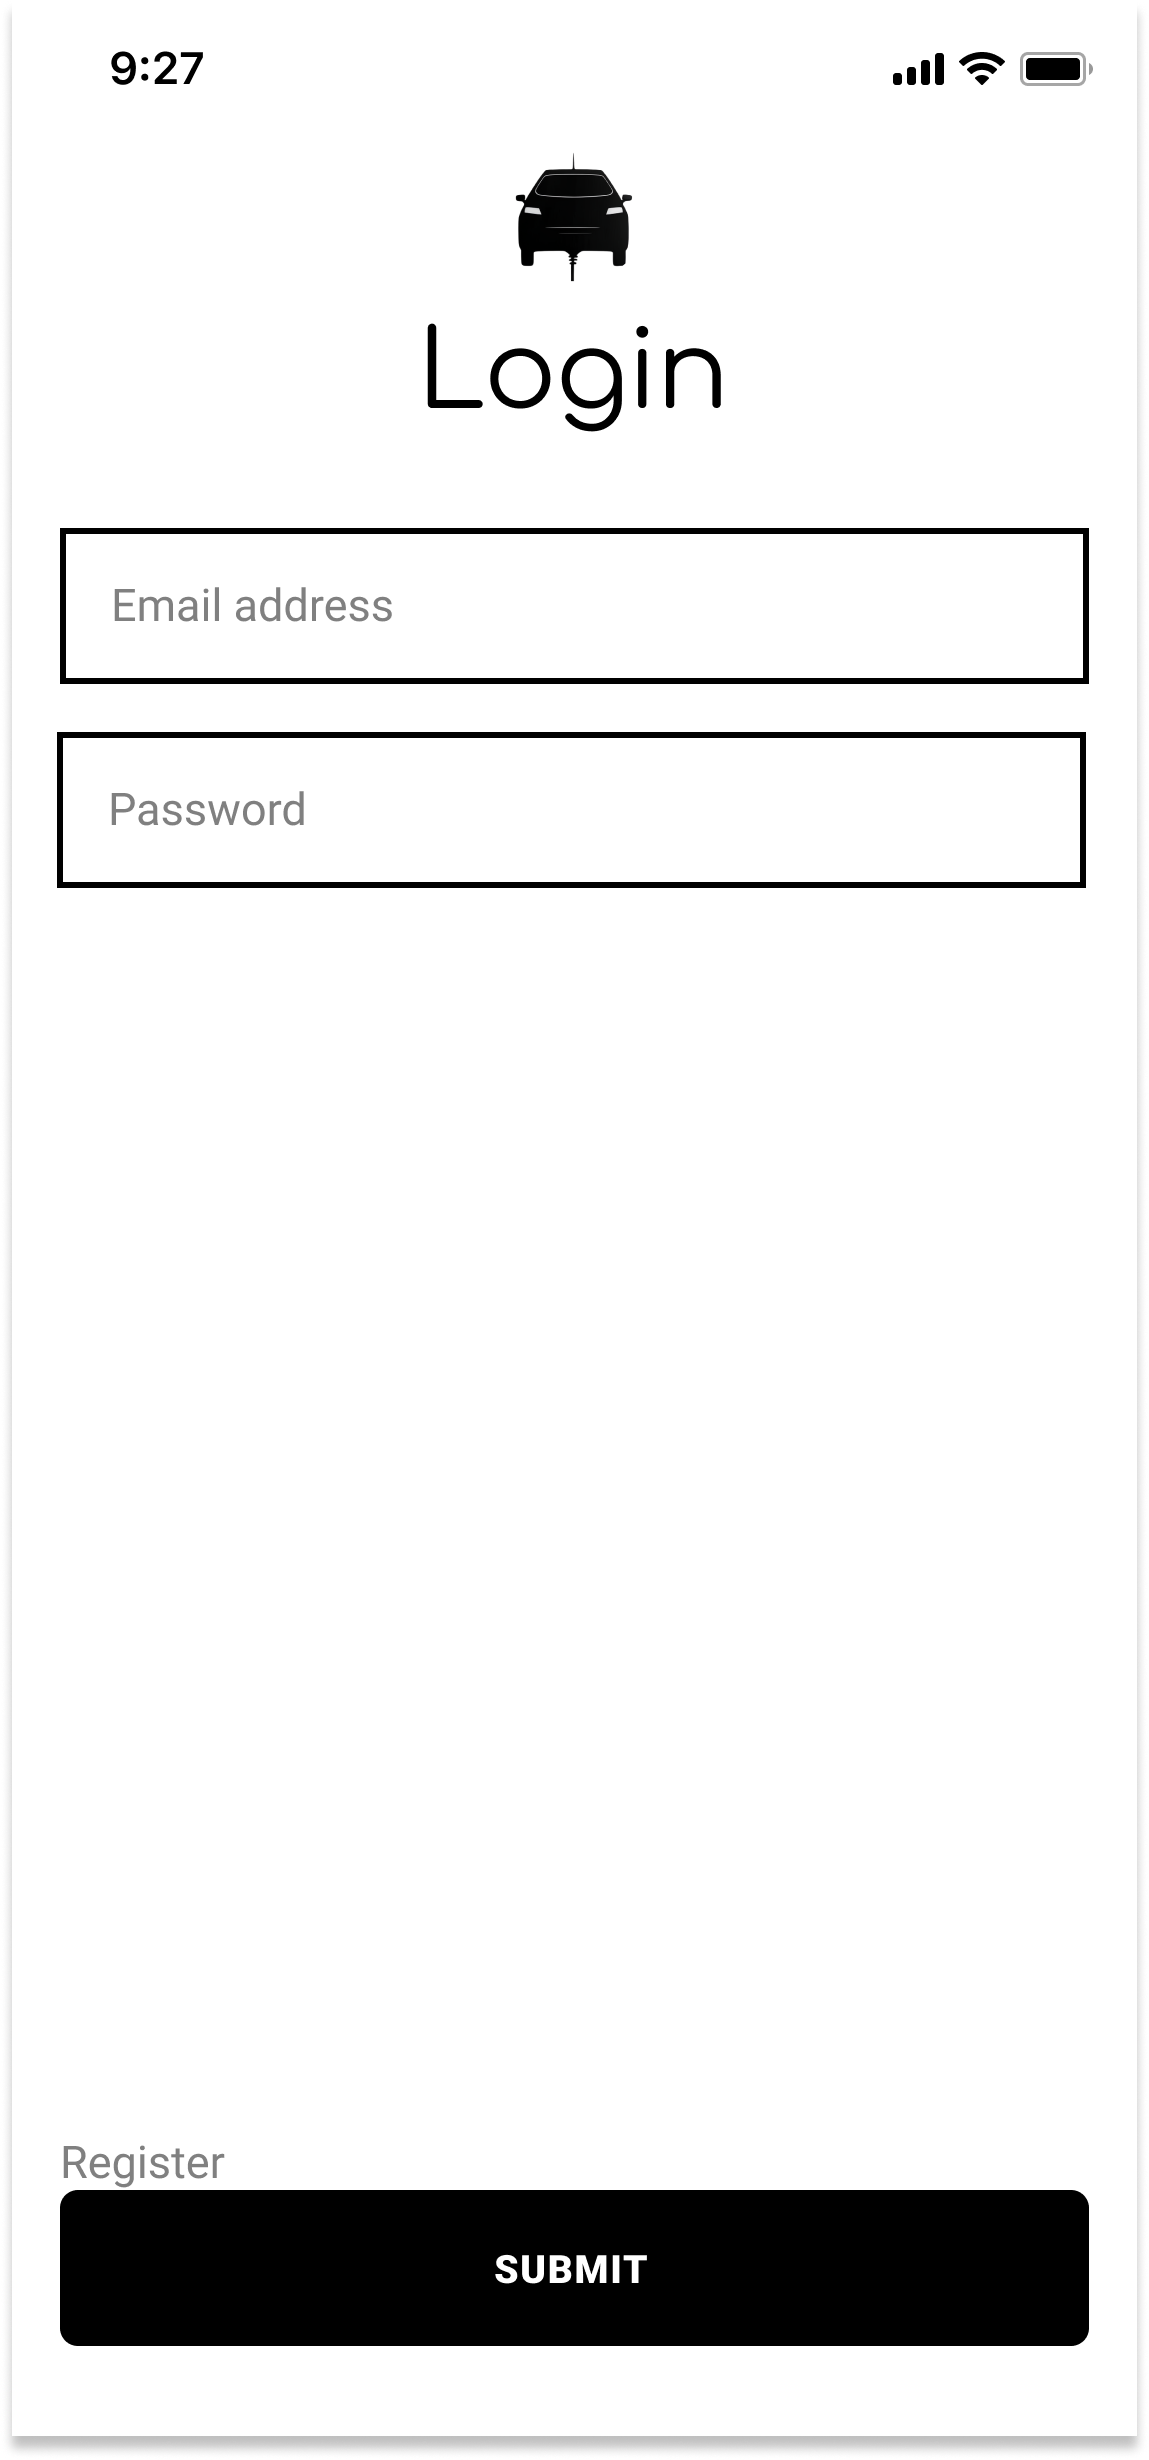
\includegraphics[keepaspectratio, height=15cm]{Mockup/UserAppInterface/Login.png}
    \caption{User Logs in}
    \label{fig:Login}
\end{figure}
The first time the user opens the app he/her is prompted to log in by inserting email and password in the corresponding field and pressing the submit button. If the information provided are correct the \hyperref[fig:Search]{search station page} is displayed; otherwise the \hyperref[fig:FailedLogin]{failed login page} is shown.\\
The user can press the register button to open the \hyperref[fig:Register]{register page}.
\begin{figure}[H]
    \centering
    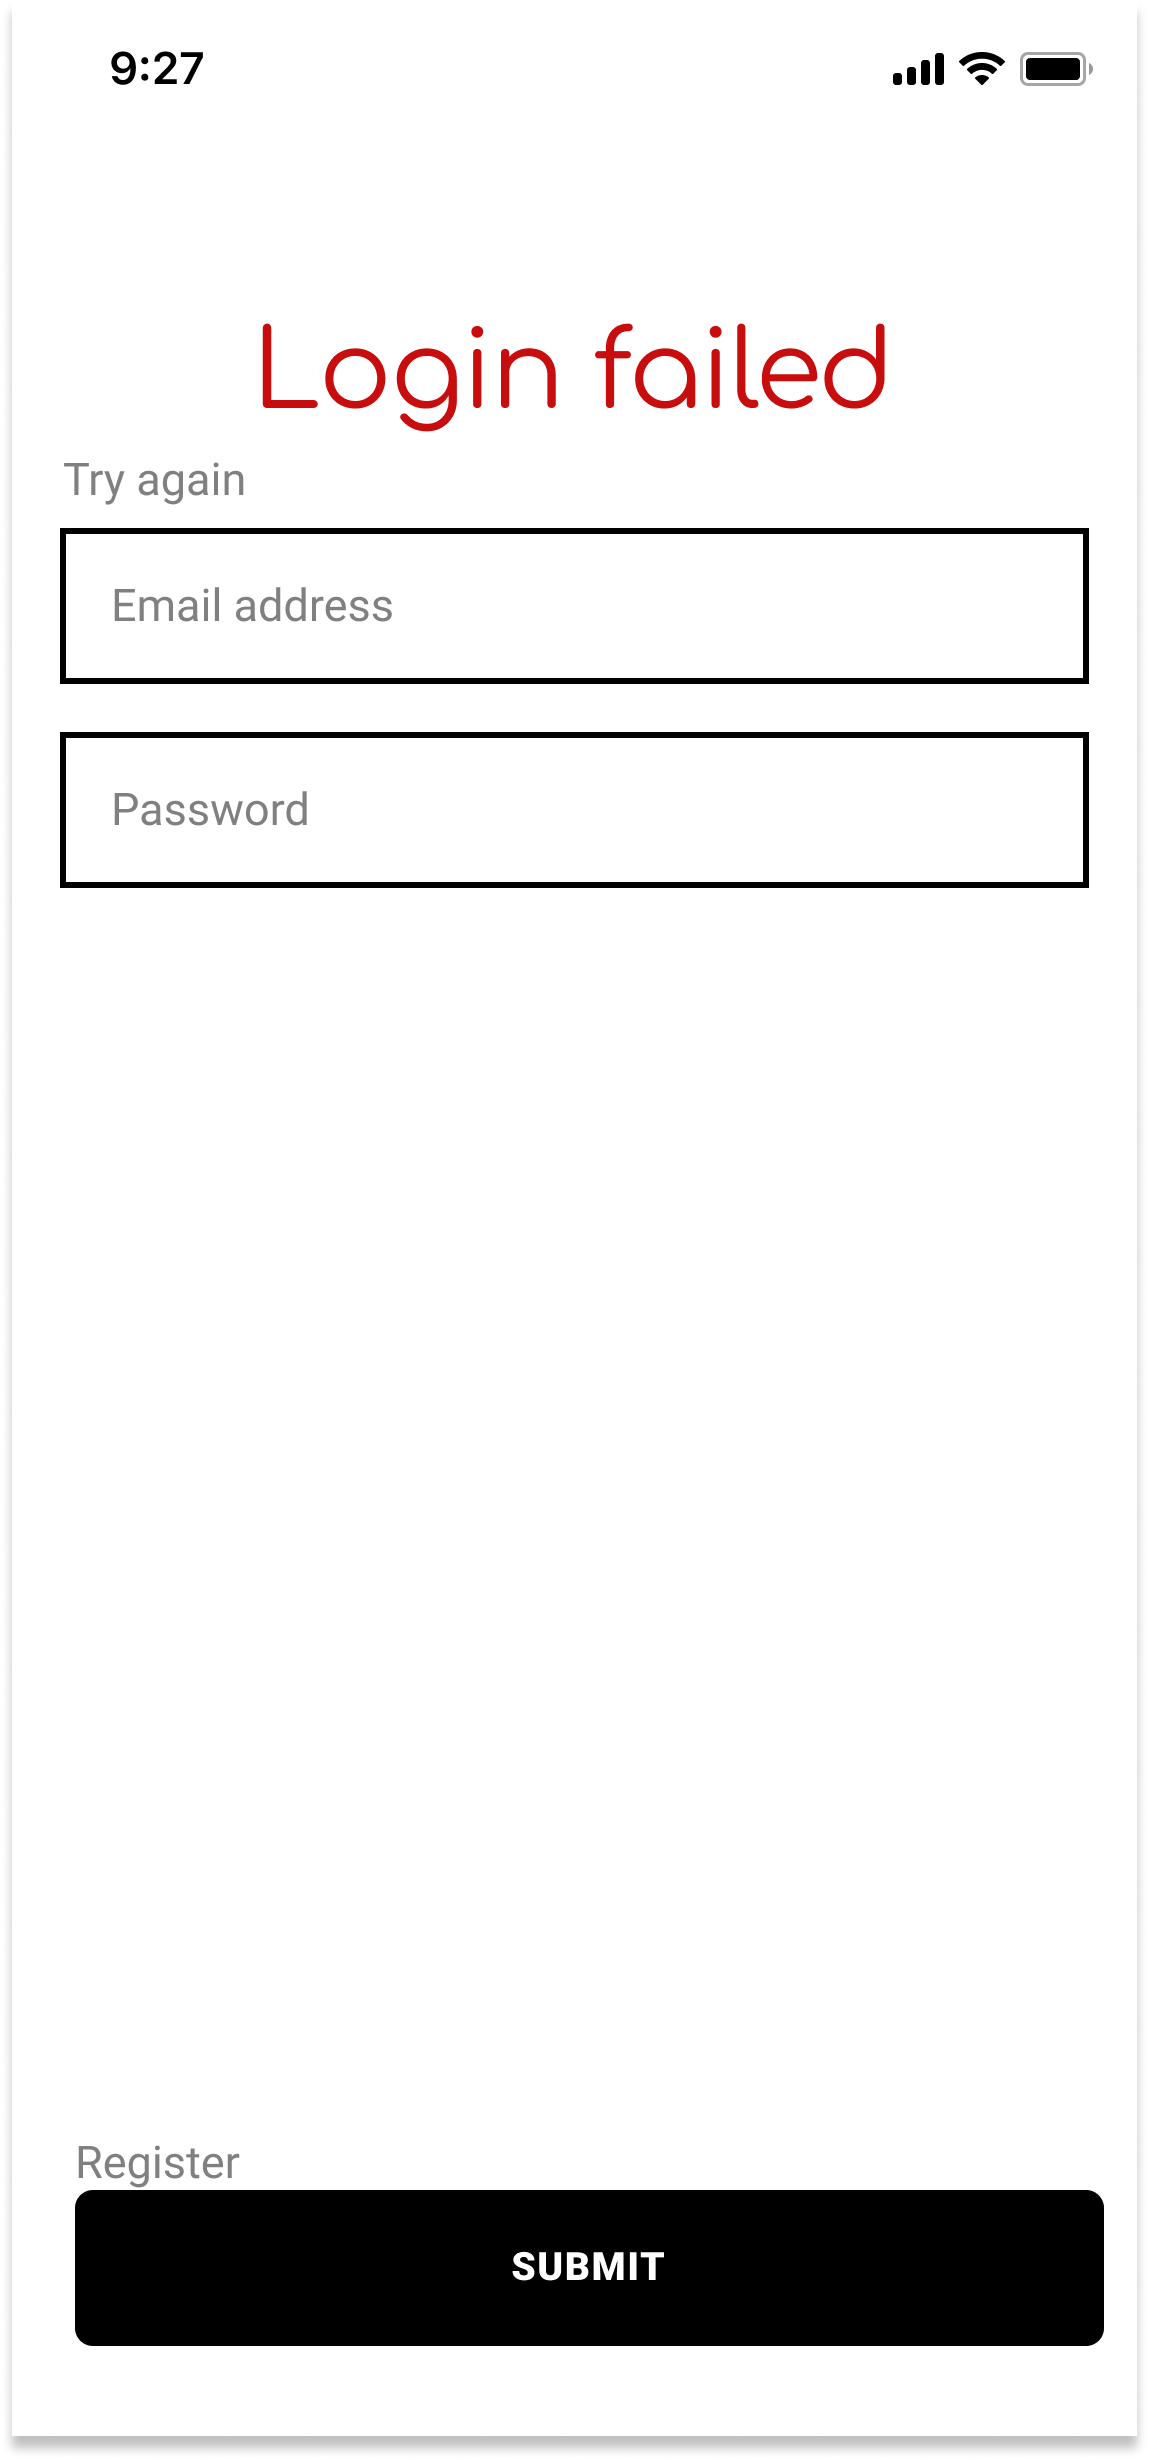
\includegraphics[keepaspectratio, height=15cm]{Mockup/UserAppInterface/Failed Login.png}
    \caption{Wrong Credential}
    \label{fig:FailedLogin}
\end{figure}
If the user has inserted the wrong email or password he/she can retry it in this page, otherwise the user can press the Sign Up button to open the \hyperref[fig:Register]{register page}.


\subsubsection{Register}
\begin{figure}[H]
    \centering
    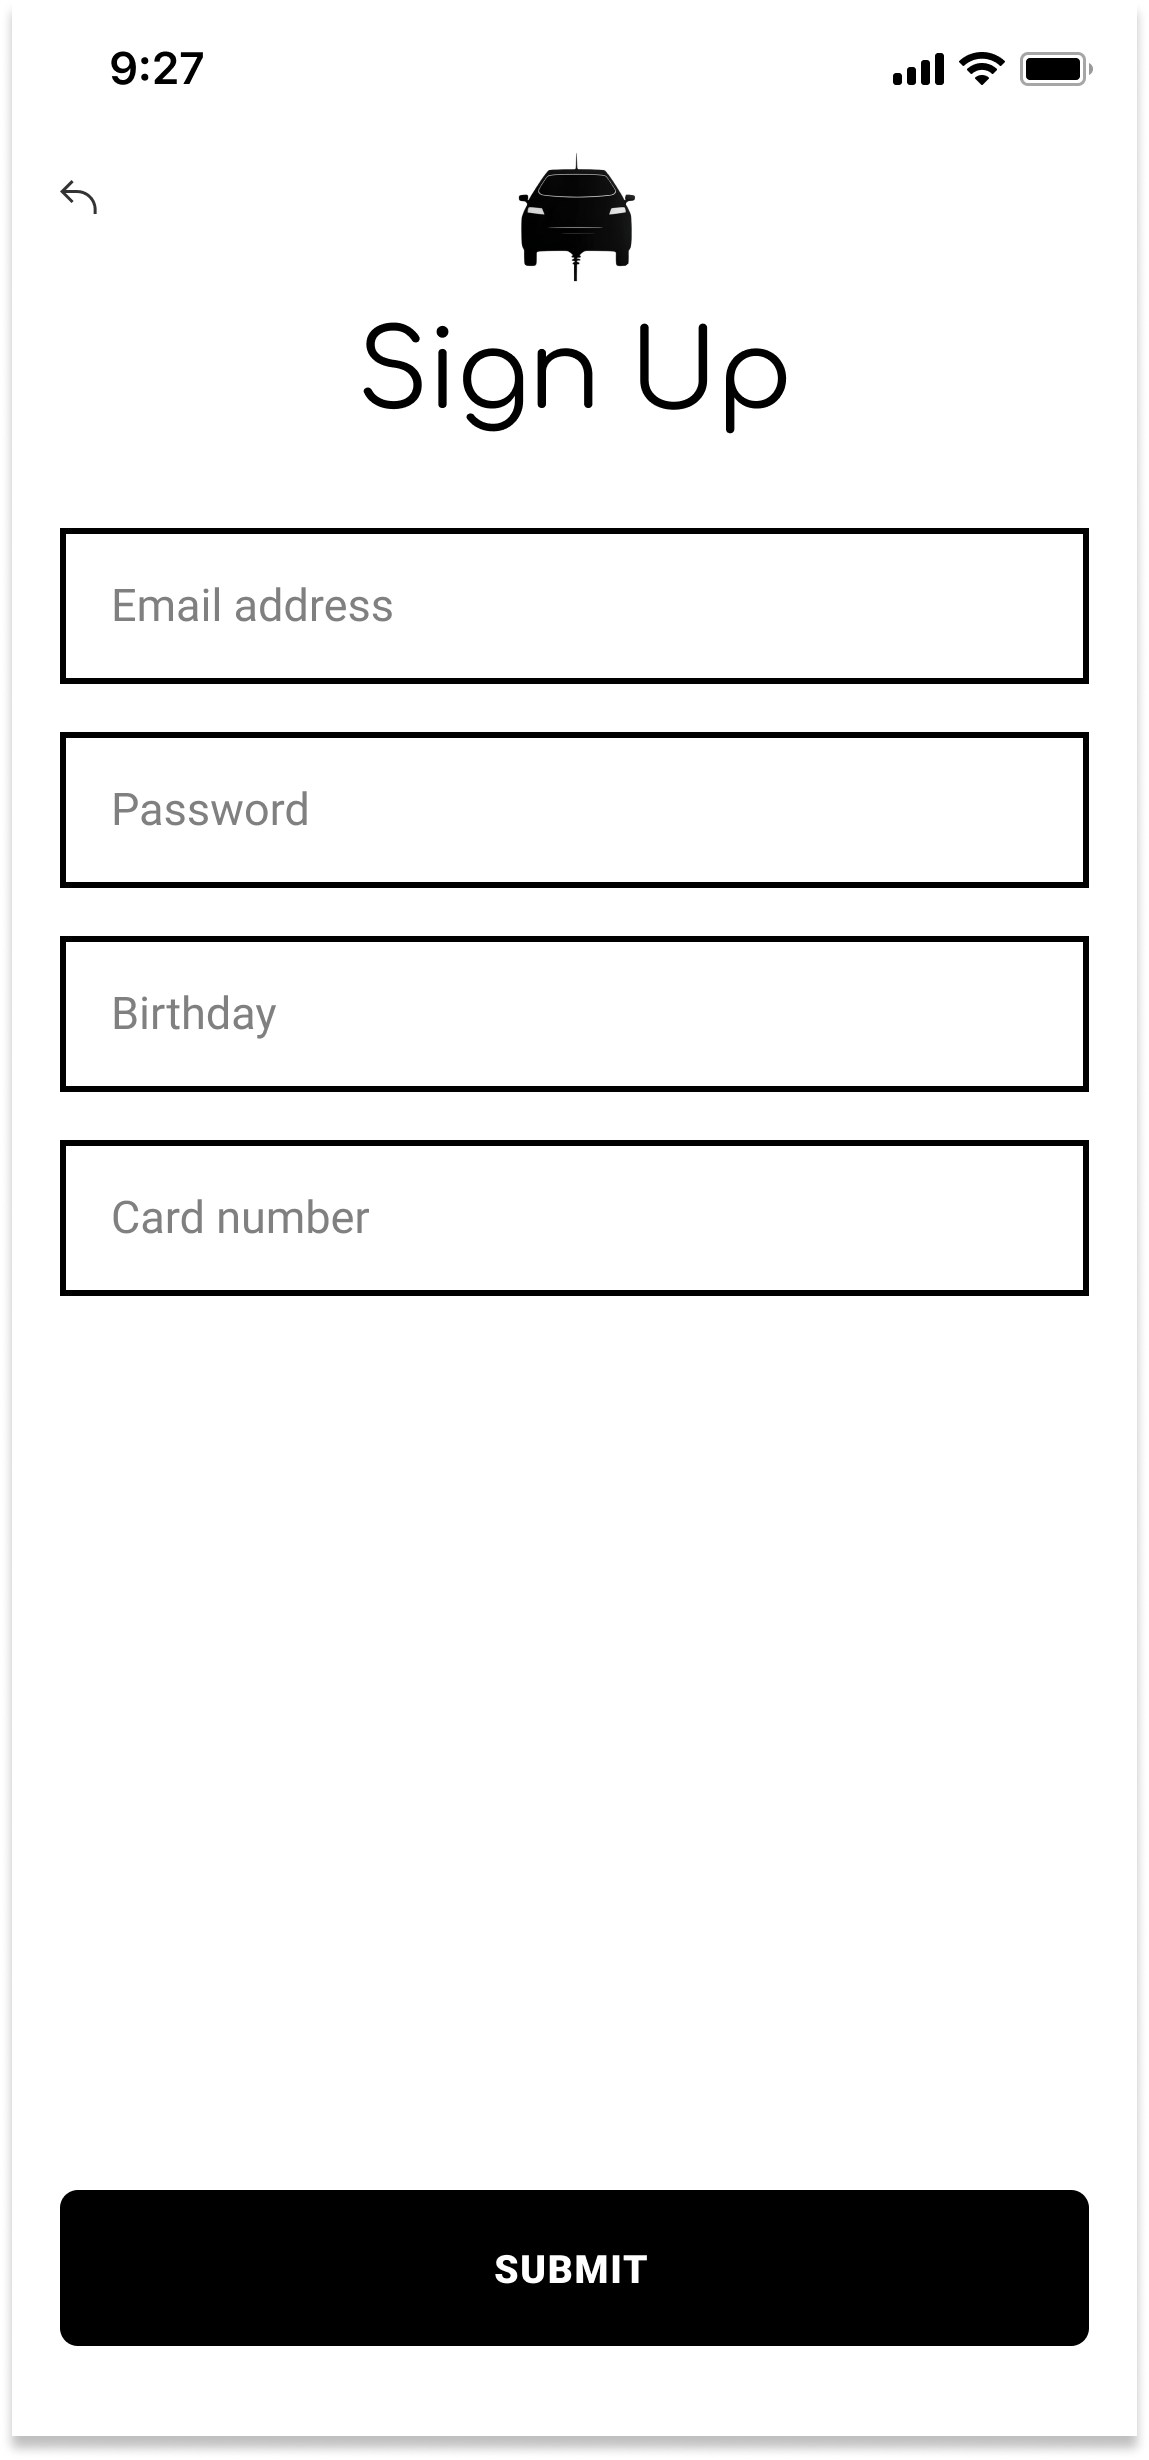
\includegraphics[keepaspectratio, height=15cm]{Mockup/UserAppInterface/Register.png}
    \caption{User Register}
    \label{fig:Register}
\end{figure}
If the user has not already registered himself/herself he/her can do it here by inserting the right data in the corresponding fields and pressing the submit button.
An email will be sent to the user with a link within, clicking the link will open the app displaying the \hyperref[fig:ConfirmReg]{confirmation page} completing the registration procedure.\\
If the user wants to return to the \hyperref[fig:Login]{login page} he can do so by pressing the backward arrow in the top left corner.
\begin{figure}[H]
    \centering
    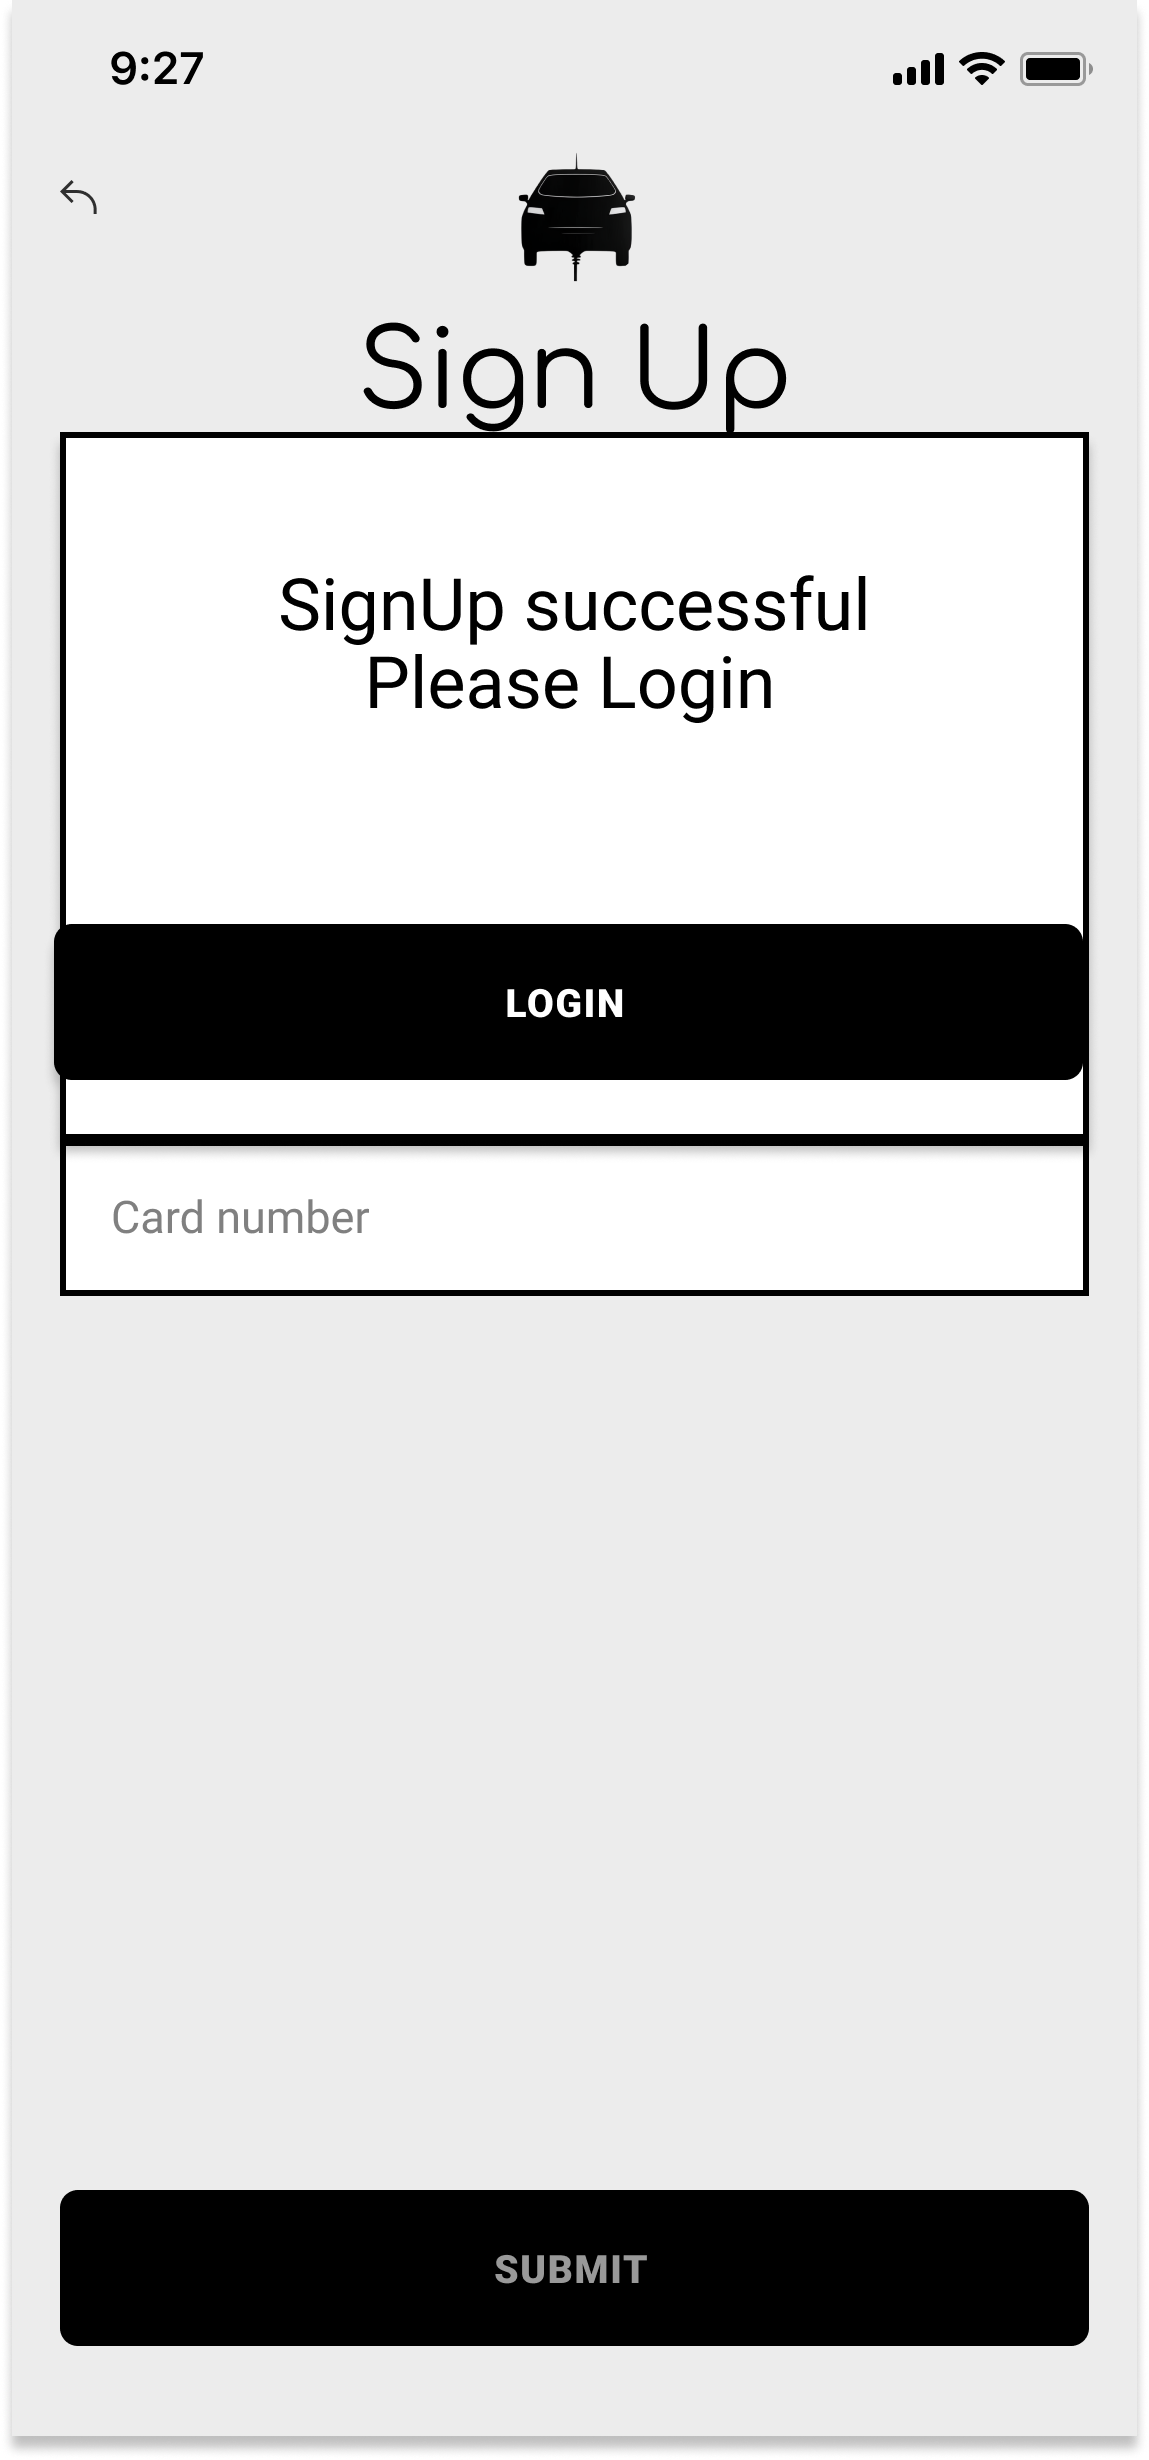
\includegraphics[keepaspectratio, height=15cm]{Mockup/UserAppInterface/Registration Succesful.png}
    \caption{User Finish Registering}
    \label{fig:ConfirmReg}
\end{figure}
once this page is displayed the user has to log in by clicking the log in button which opens the \hyperref[fig:Login]{login page}.
\subsubsection{Search a Station}
At any screen shown in this section the user can press the car logo at the top to load the \hyperref[fig:myCharges]{manage charges page}
\begin{figure}[H]
    \centering
    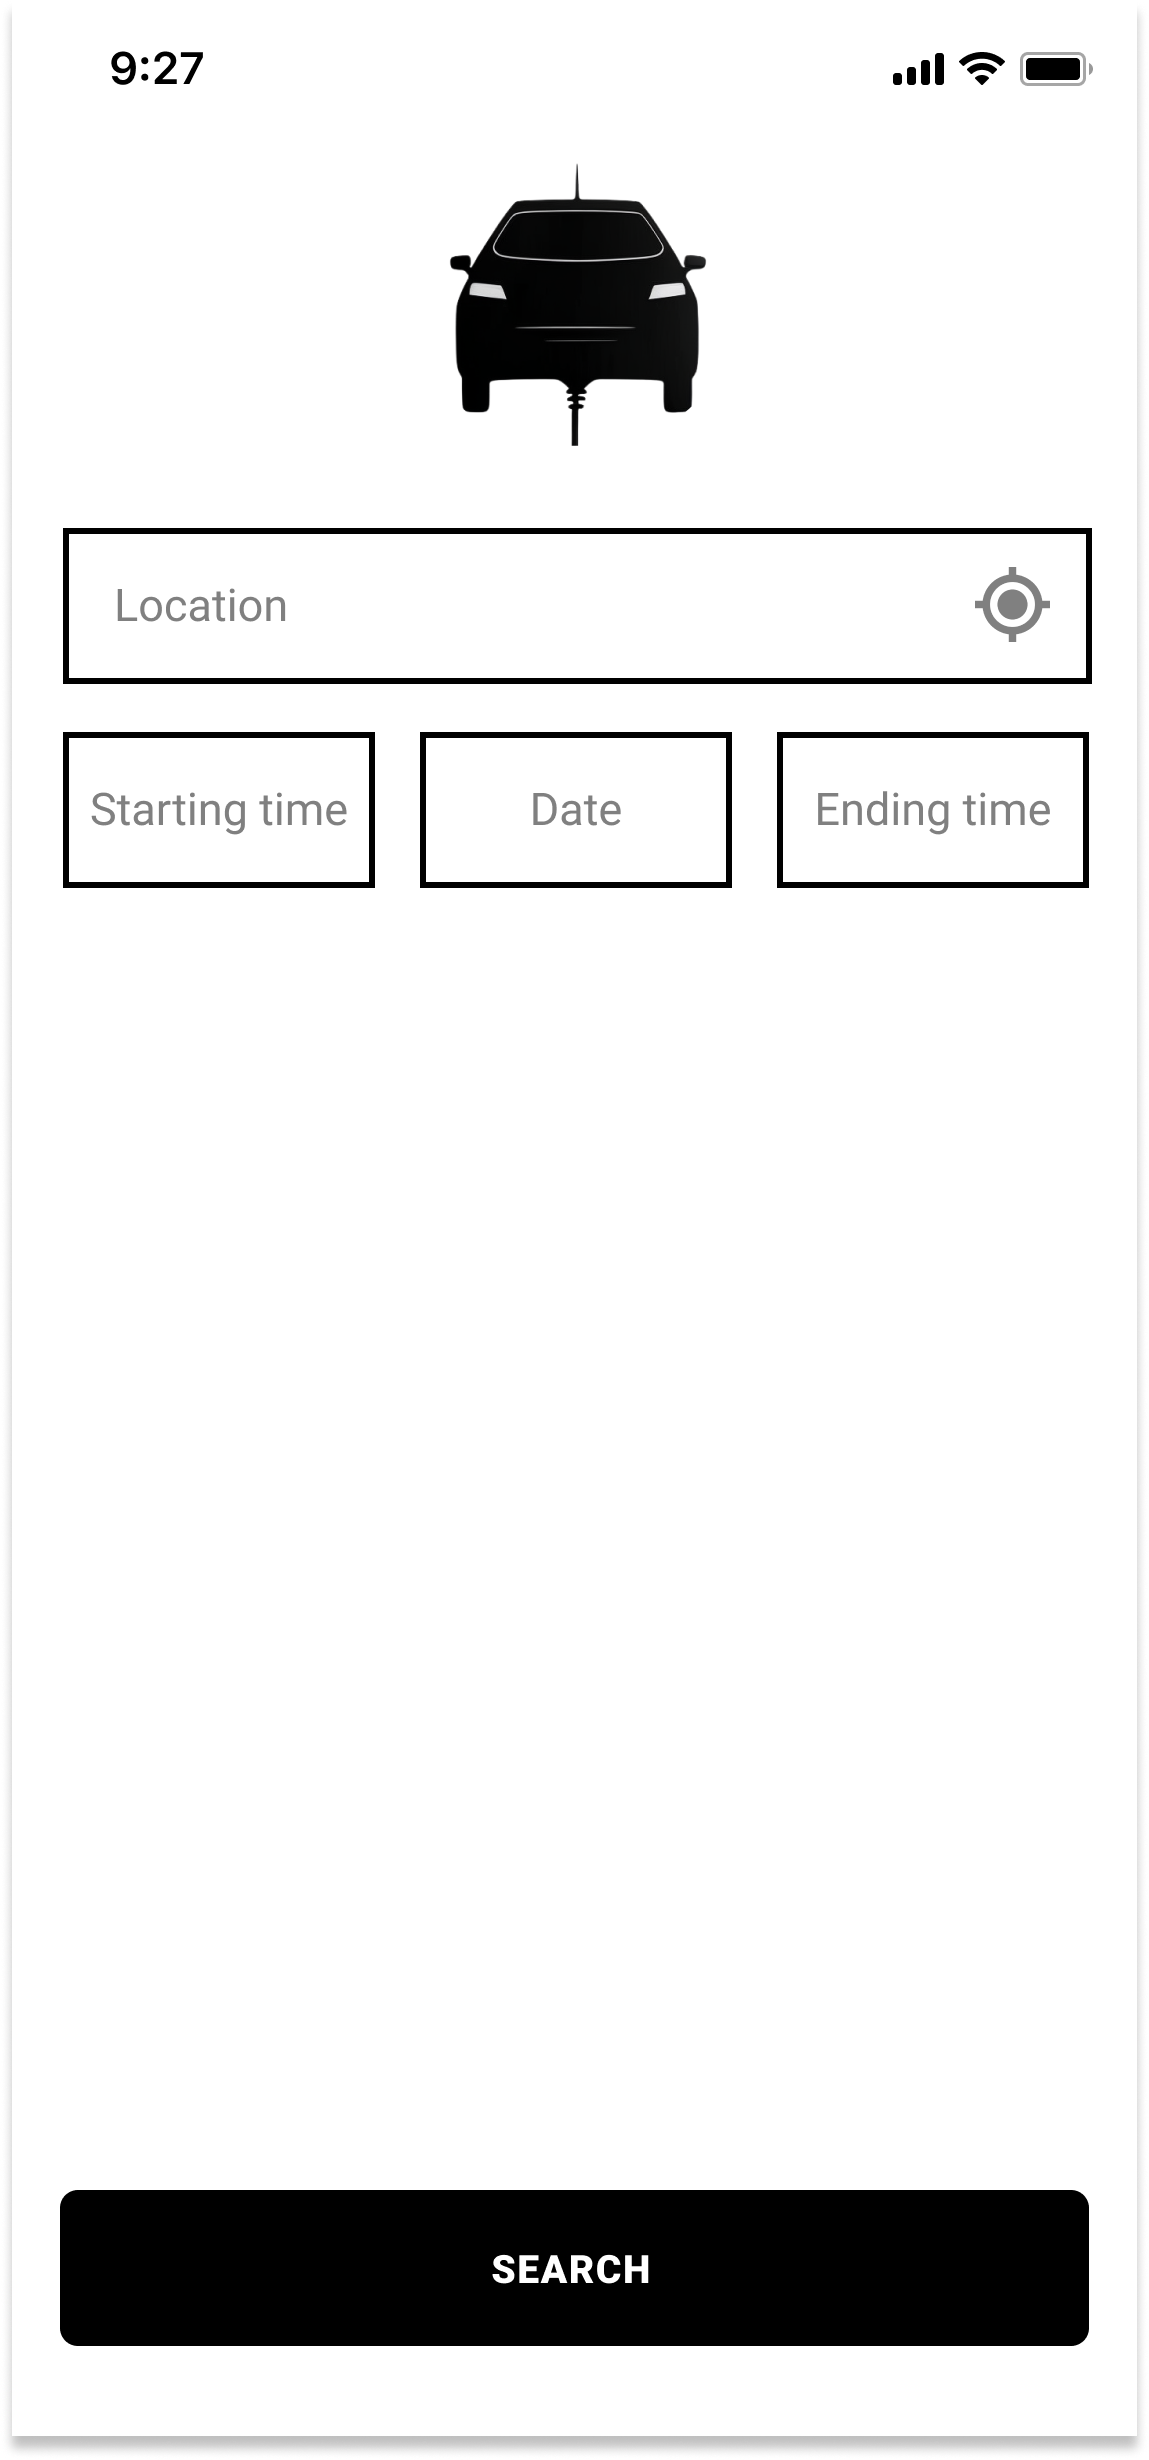
\includegraphics[keepaspectratio, height=15cm]{Mockup/UserAppInterface/Station Search.png}
    \caption{User Search for Stations}
    \label{fig:Search}
\end{figure}
In this section the user can search for stations by inserting the location, the starting and ending time for the charge. By pressing the location icon the user can automatically use his current location.
Once the data are inserted the user can press Search to advance to the \hyperref[fig:Results]{results page}.
\begin{figure}[H]
    \centering
    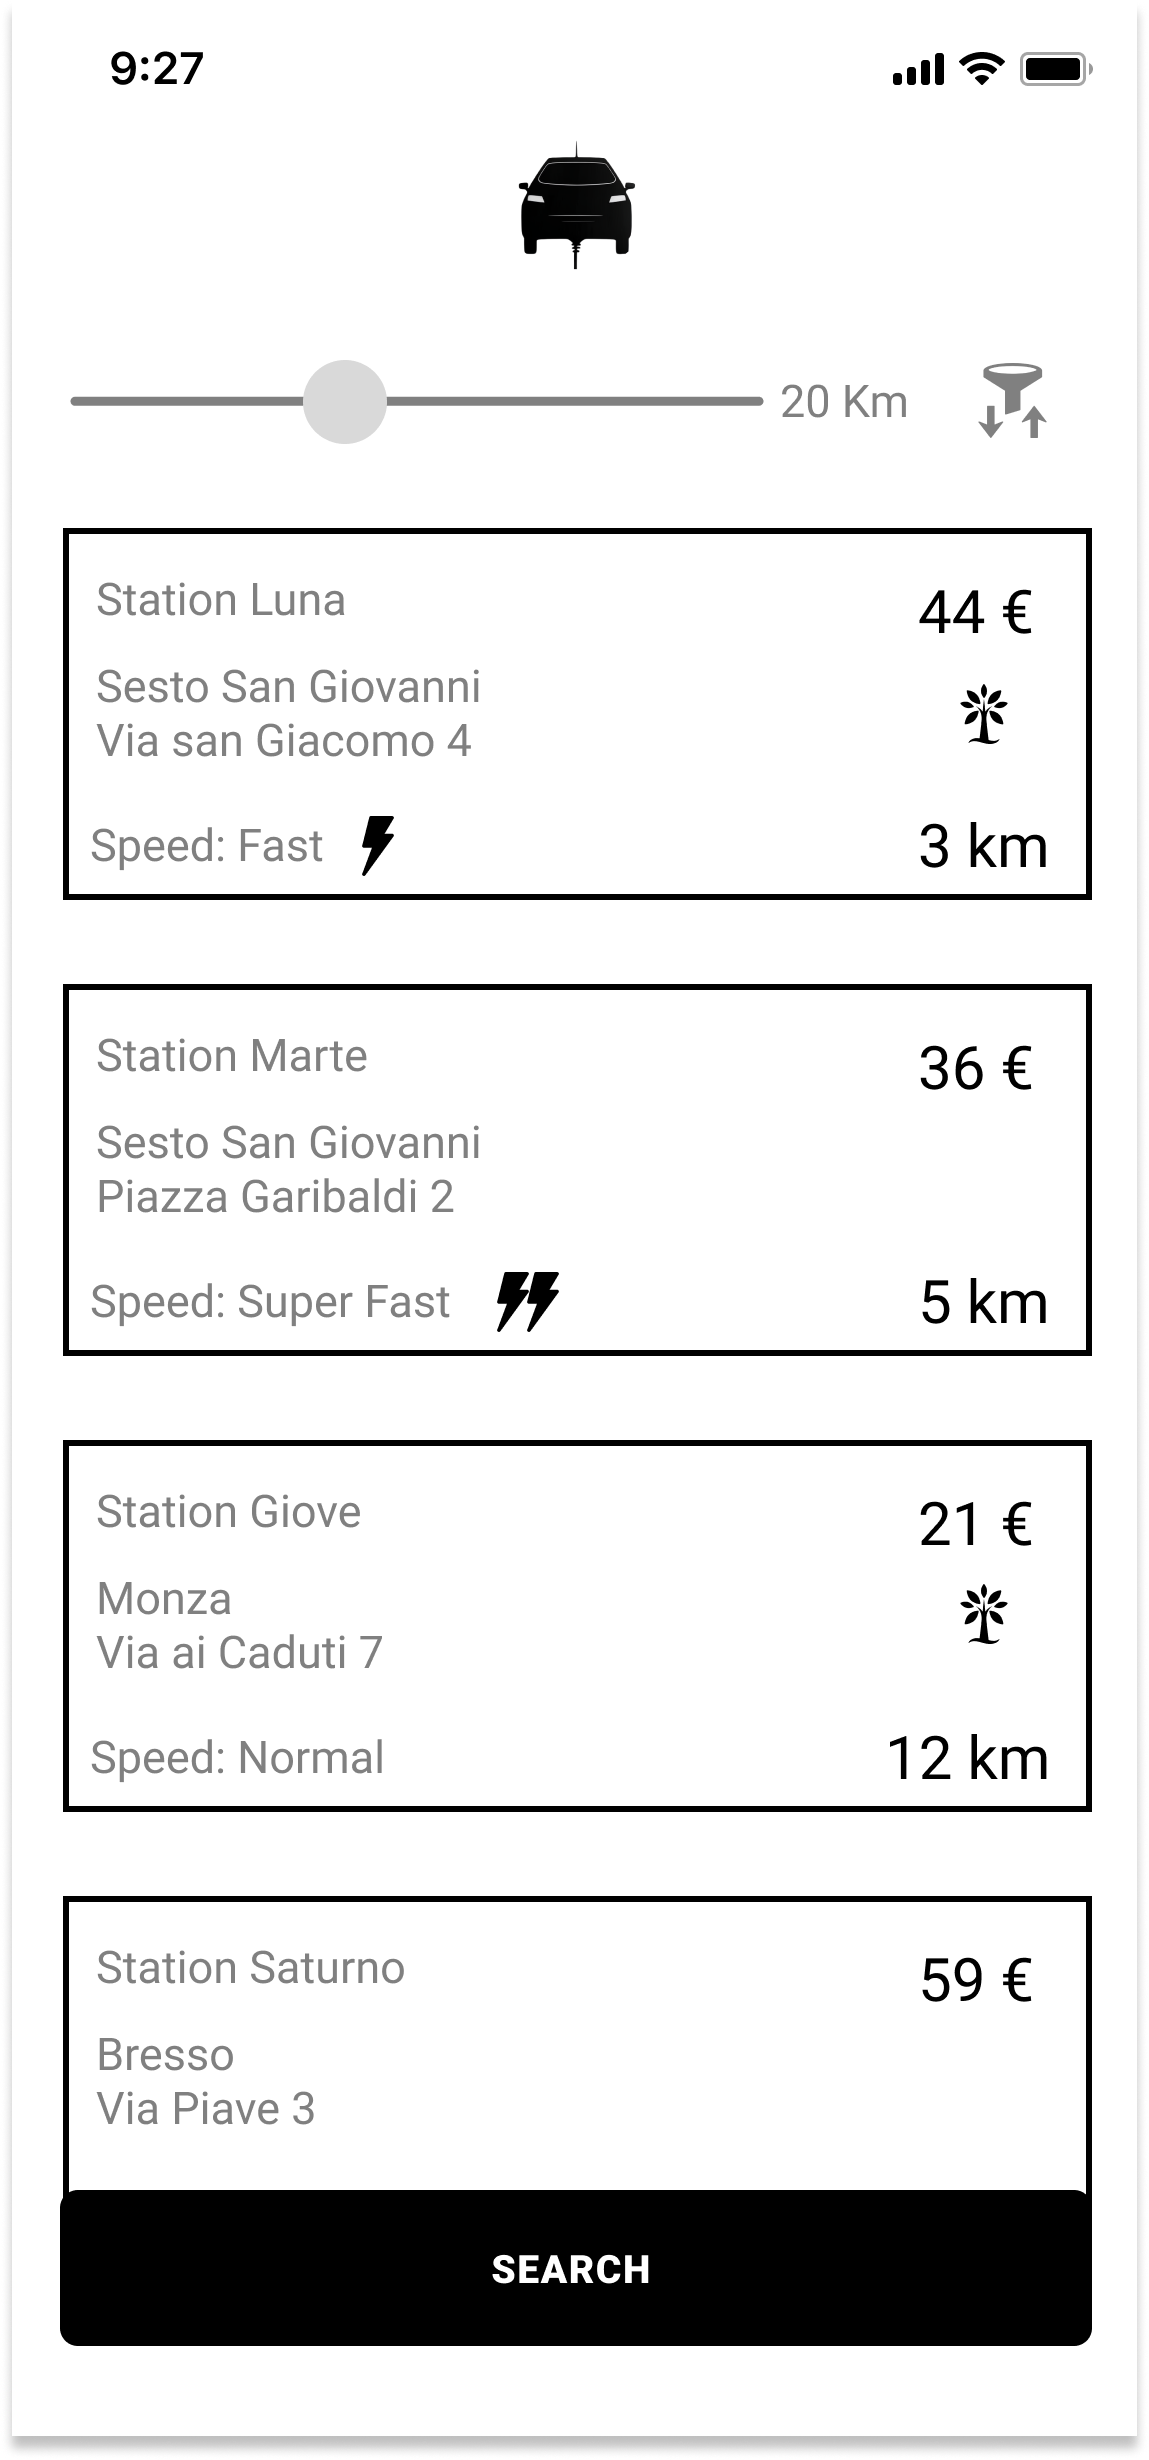
\includegraphics[keepaspectratio, height=15cm]{Mockup/UserAppInterface/Results.png}
    \caption{Search results}
    \label{fig:Results}
\end{figure}
Here the user is shown the results of the search, using the slider on top the user can change the radius of search from the given position, at the right of the slide the selected distance is shown; at the most right the filter icon is displayed, if pressed the \hyperref[fig:Filters]{filter popup} is showed.\\
A list of station with their details is displayed (station name, location, speed, distance from selected location and price of the charge), clicking on a station opens that \hyperref[fig:StationDetails]{station details page}. Pressing the Search button allow the user to make another search trough the \hyperref[fig:Search]{search station page}.
\begin{figure}[H]
    \centering
    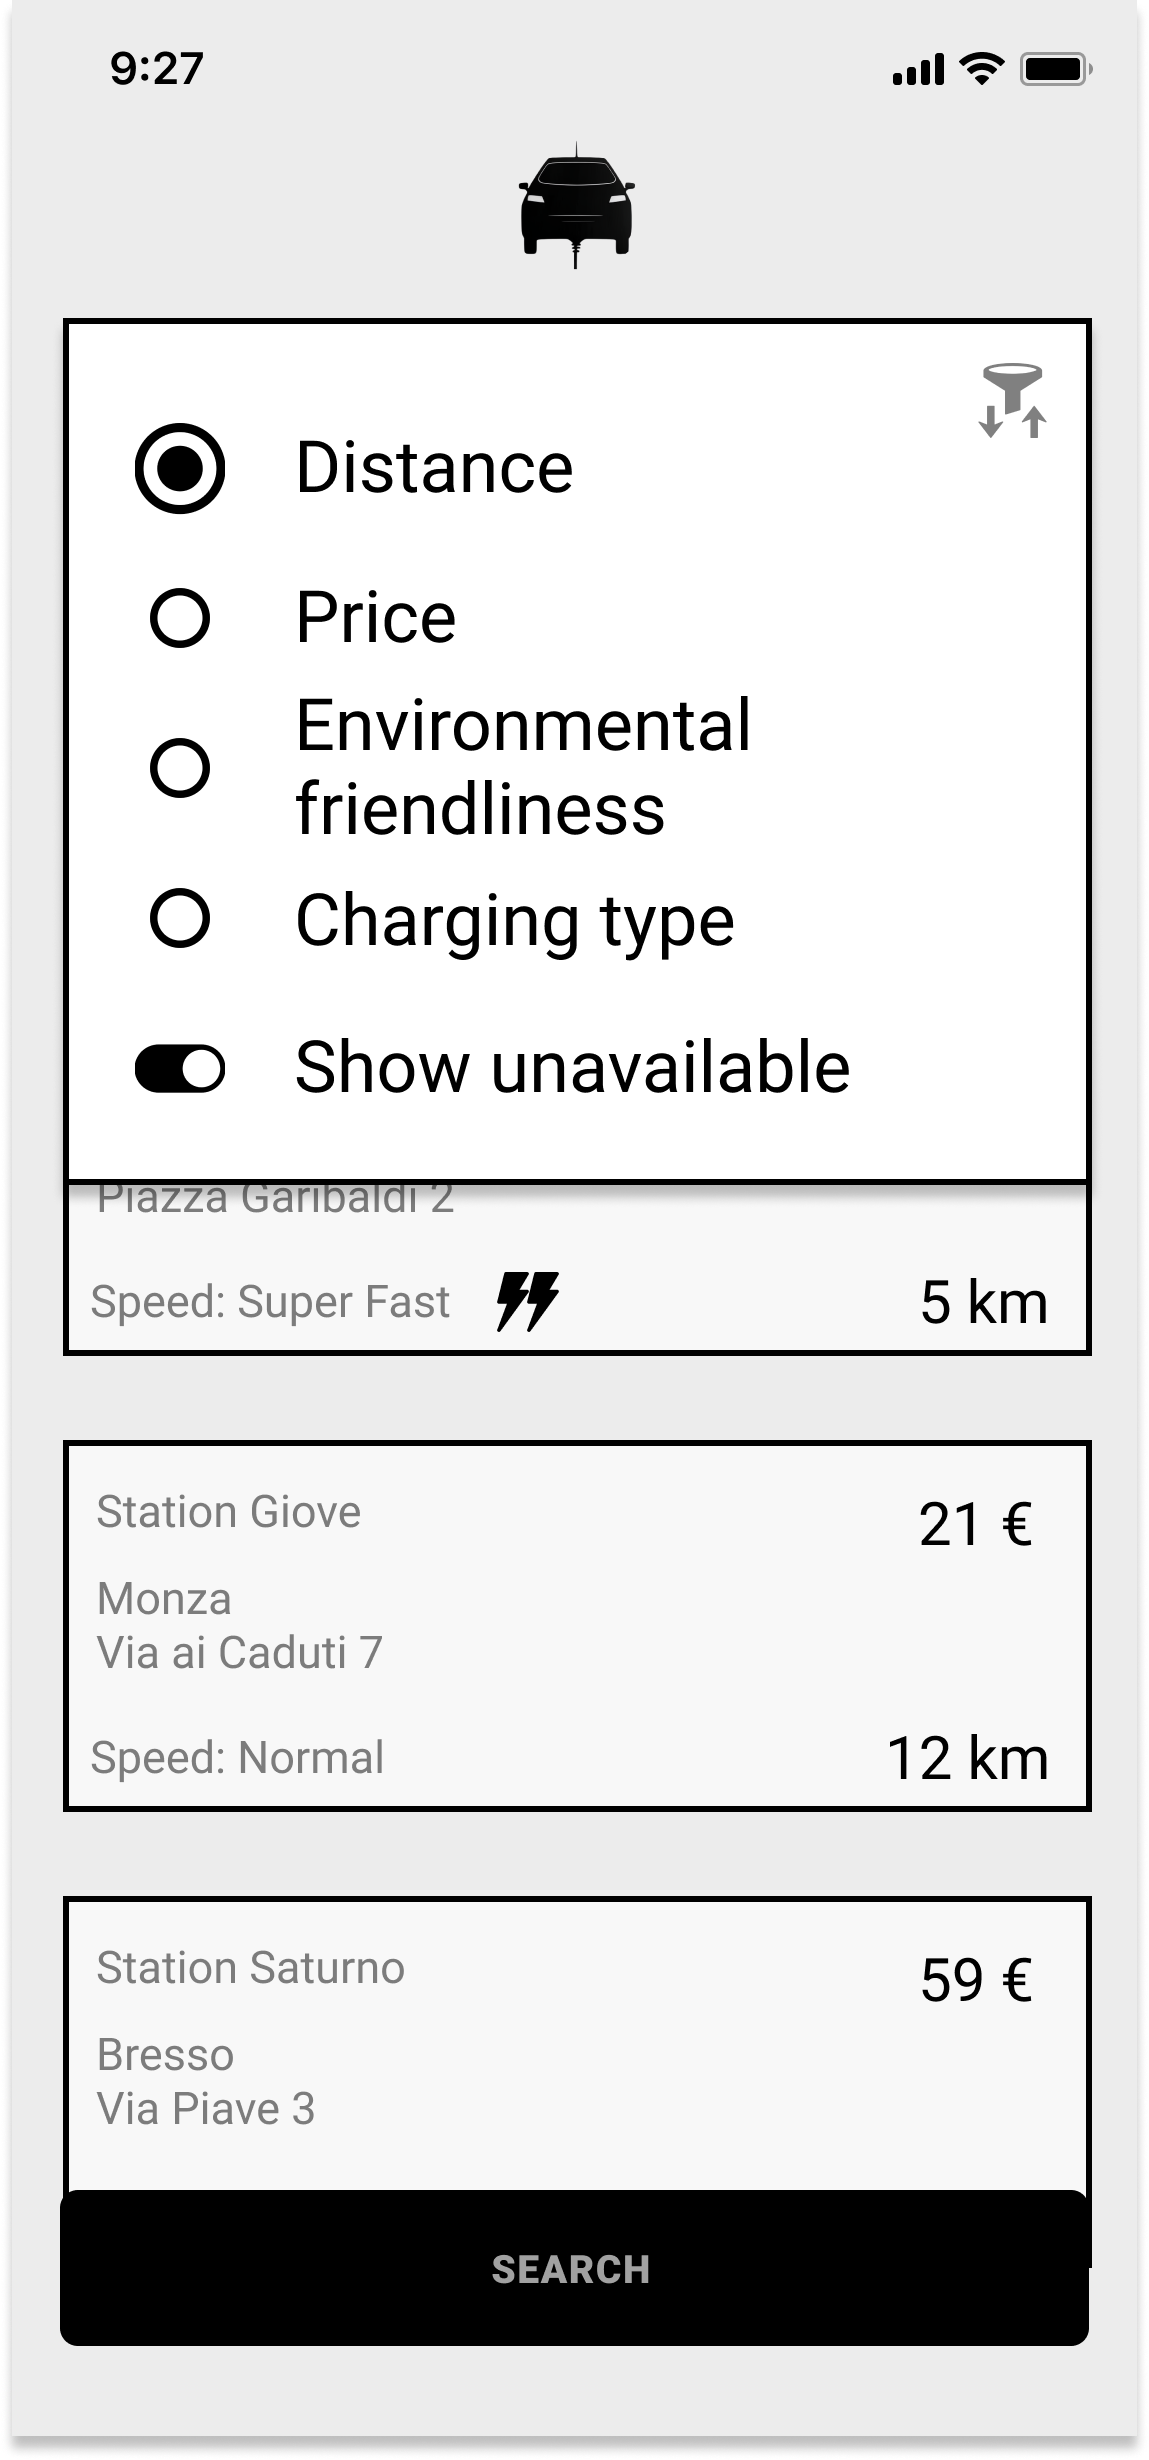
\includegraphics[keepaspectratio, height=15cm]{Mockup/UserAppInterface/Filter Menu.png}
    \caption{User Filters the Results}
    \label{fig:Filters}
\end{figure}
In this popup the user can select whether to sort the results by distance, price, environmental friendliness or charging type via a radio button, and to show or to not show unavailable station trough the toggle.
\subsection{Select time frame}
At any screen shown in this section the user can press the car logo at the top to load the \hyperref[fig:myCharges]{manage charges page}
\begin{figure}[H]
    \centering
    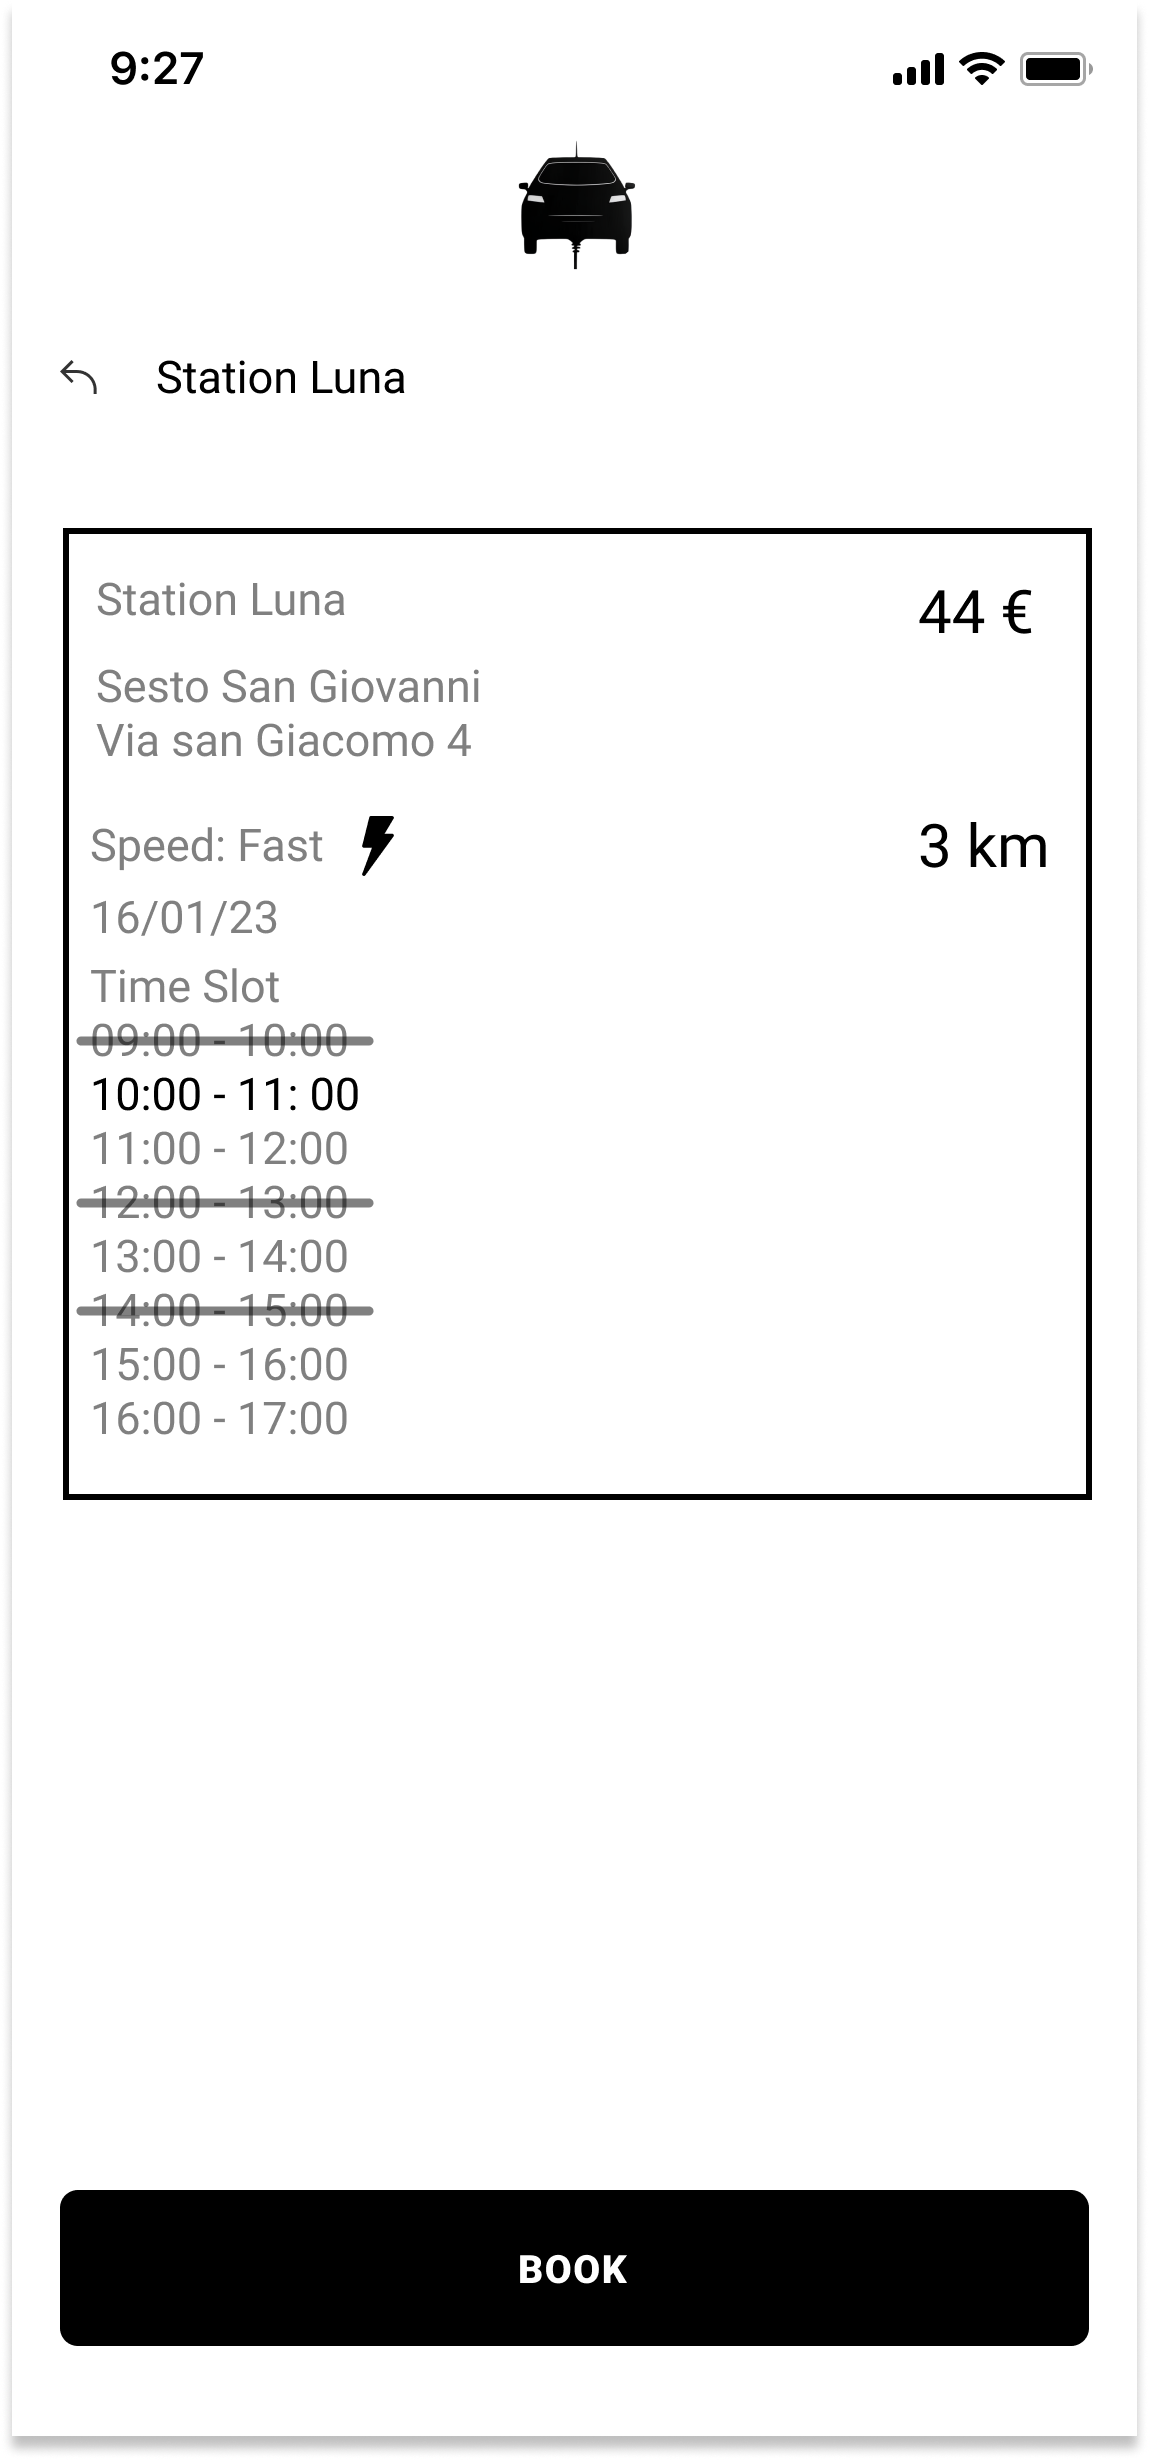
\includegraphics[keepaspectratio, height=15cm]{Mockup/UserAppInterface/Station Details.png}
    \caption{User Checks Station Details}
    \label{fig:StationDetails}
\end{figure}
Here the user can select a time frame, in the center of the screen the station details and a list of possible time frames are shown; the user can select the desired time frame by tapping on it. The selected time frame is bold while unavailable time frames are crossed. Once the user has selected the time frame he/her can proceed to the booking by clicking the book button opening \hyperref[pop:Booking]{the confirmation popup}. The user can return to the \hyperref[fig:Search]{search station page} by clicking the back arrow in the top left corner.
\subsubsection{Book a Station}
\begin{figure}[H]
    \centering
    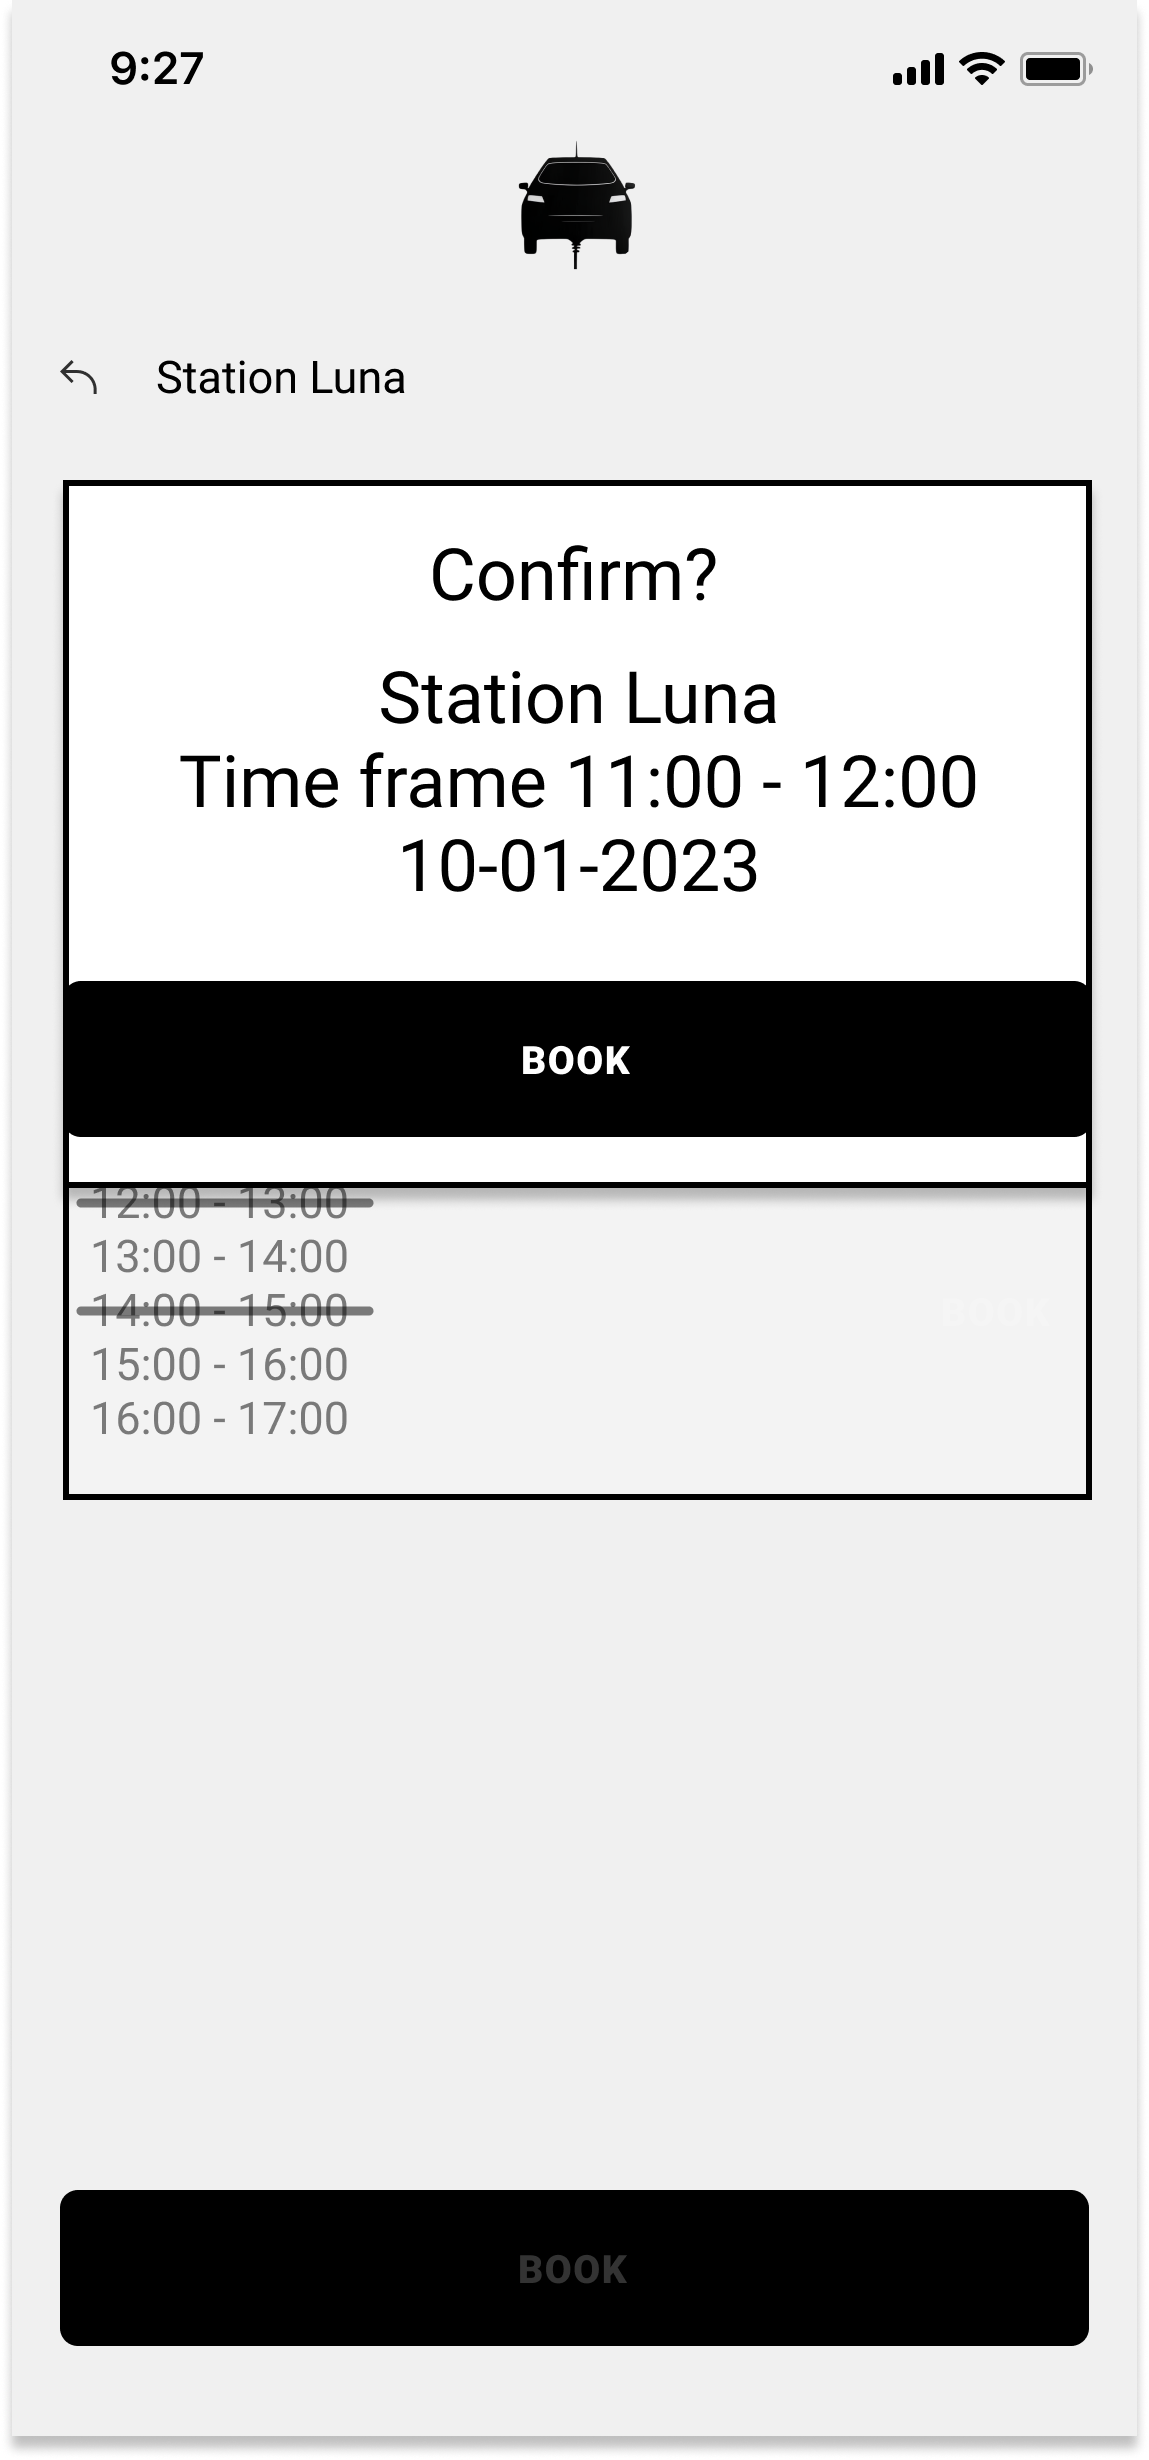
\includegraphics[keepaspectratio, height=15cm]{Mockup/UserAppInterface/Book Confirm.png}
    \caption{User Confirms the Booking}
    \label{pop:Booking}
\end{figure}
In this popup: station name, the selected date and time frame are displayed. The user can confirm the booking by pressing the Book button and opening the \hyperref[pop:BookingConfirmed]{confirmation popup}.
\begin{figure}[H]
    \centering
    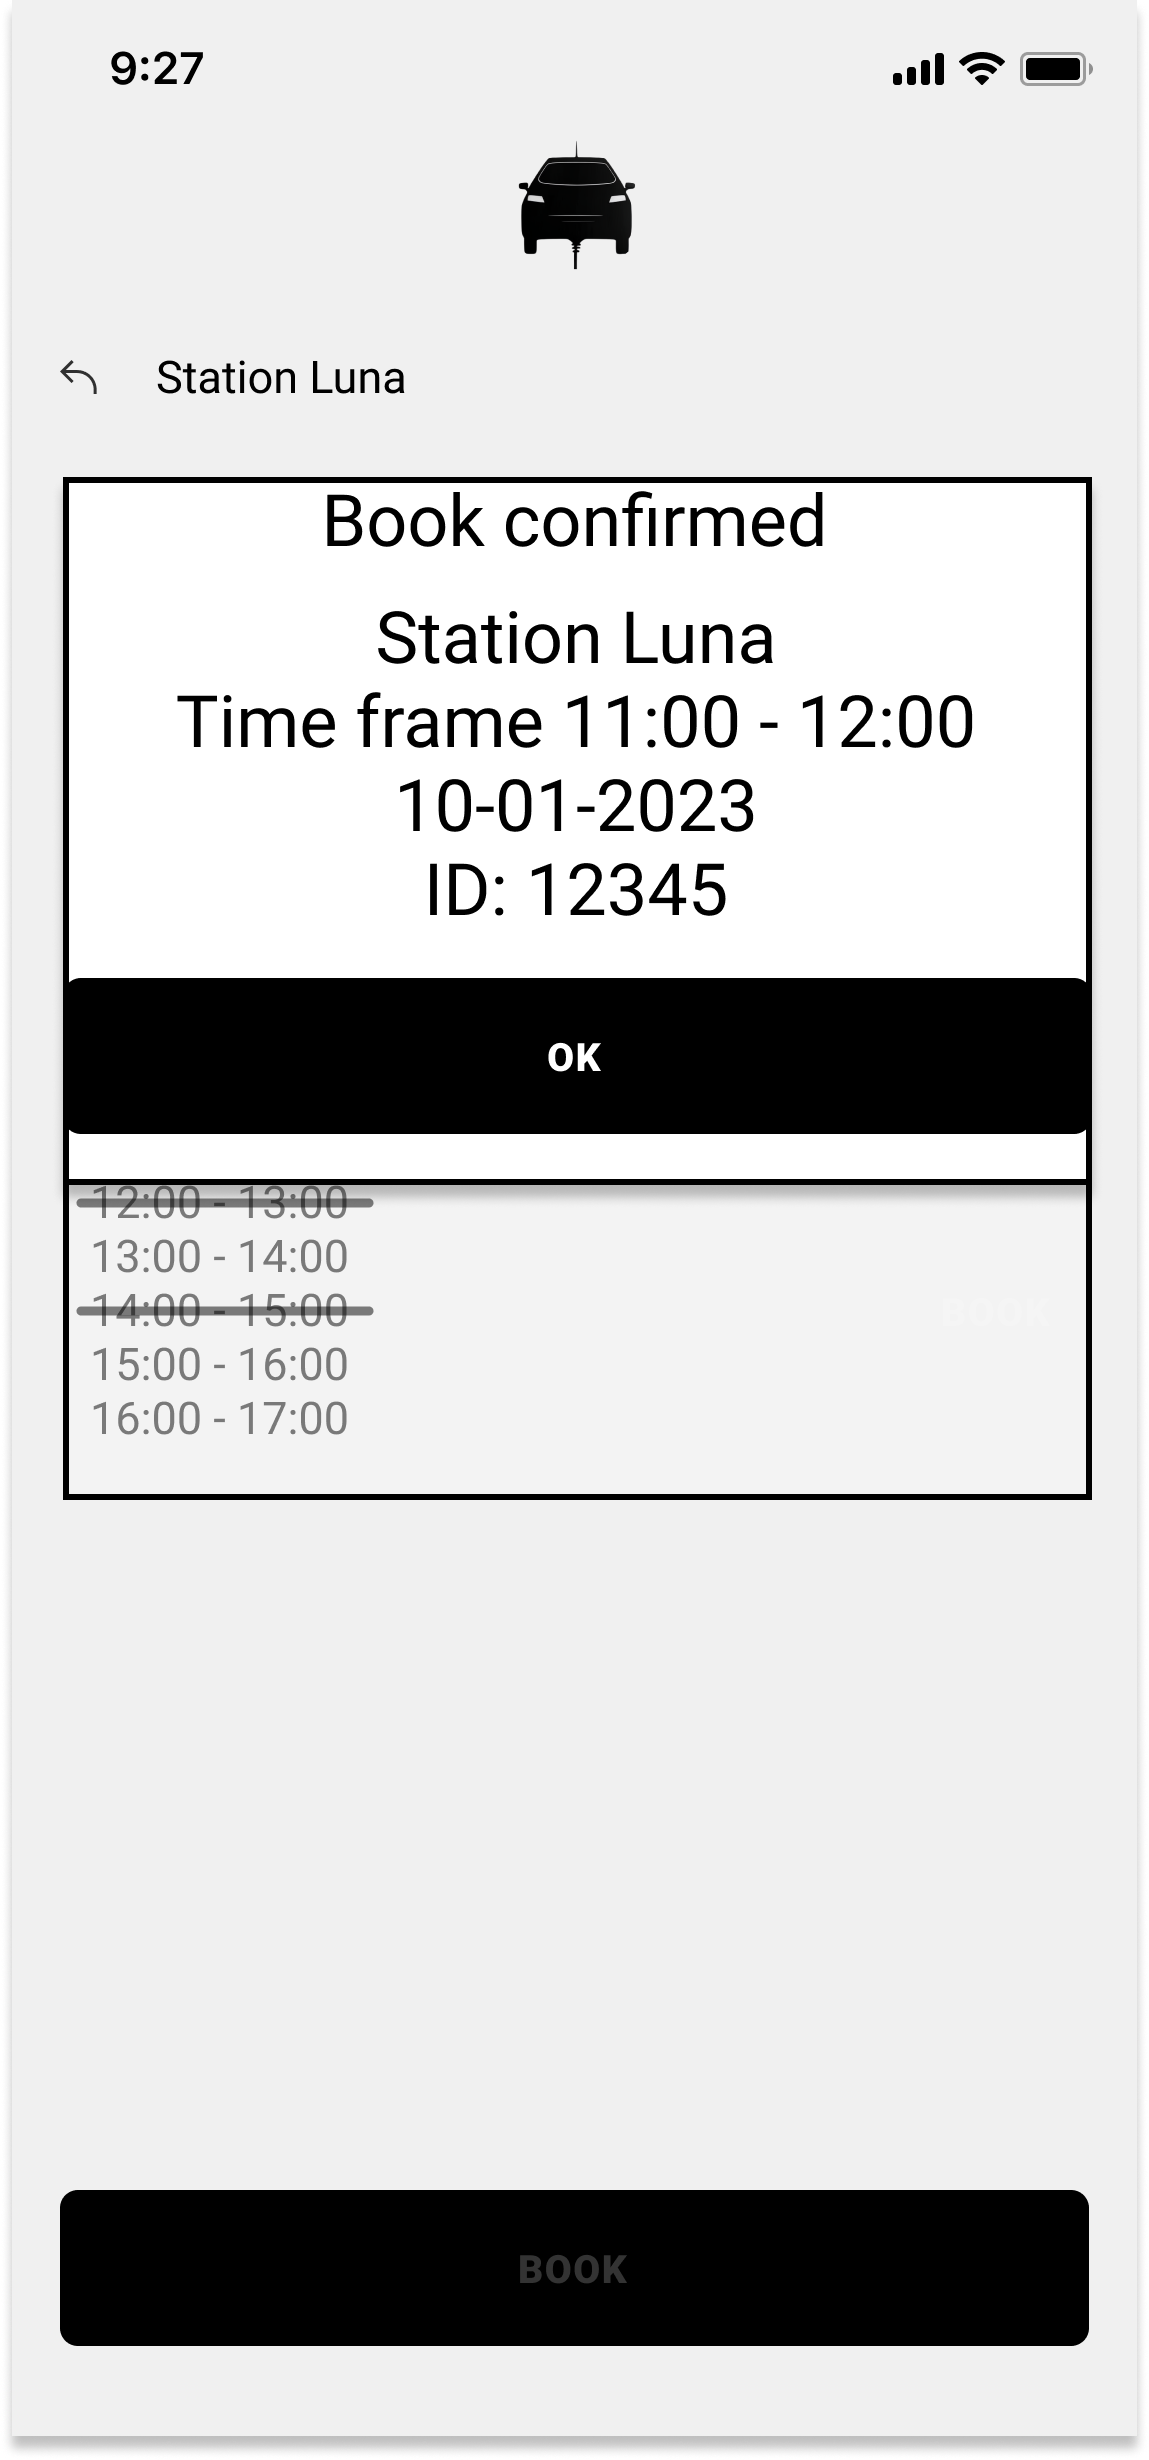
\includegraphics[keepaspectratio, height=15cm]{Mockup/UserAppInterface/Book Confirmation.png}
    \caption{User Reads Confirmation Popup}
    \label{pop:BookingConfirmed}
\end{figure}
In this popup the booking information are displayed confirming the user that the booking was successful. Pressing the ok button opens the \hyperref[fig:Search]{search station page}.
\subsubsection{Checks Booked Stations}
\begin{figure}[H]
    \centering
    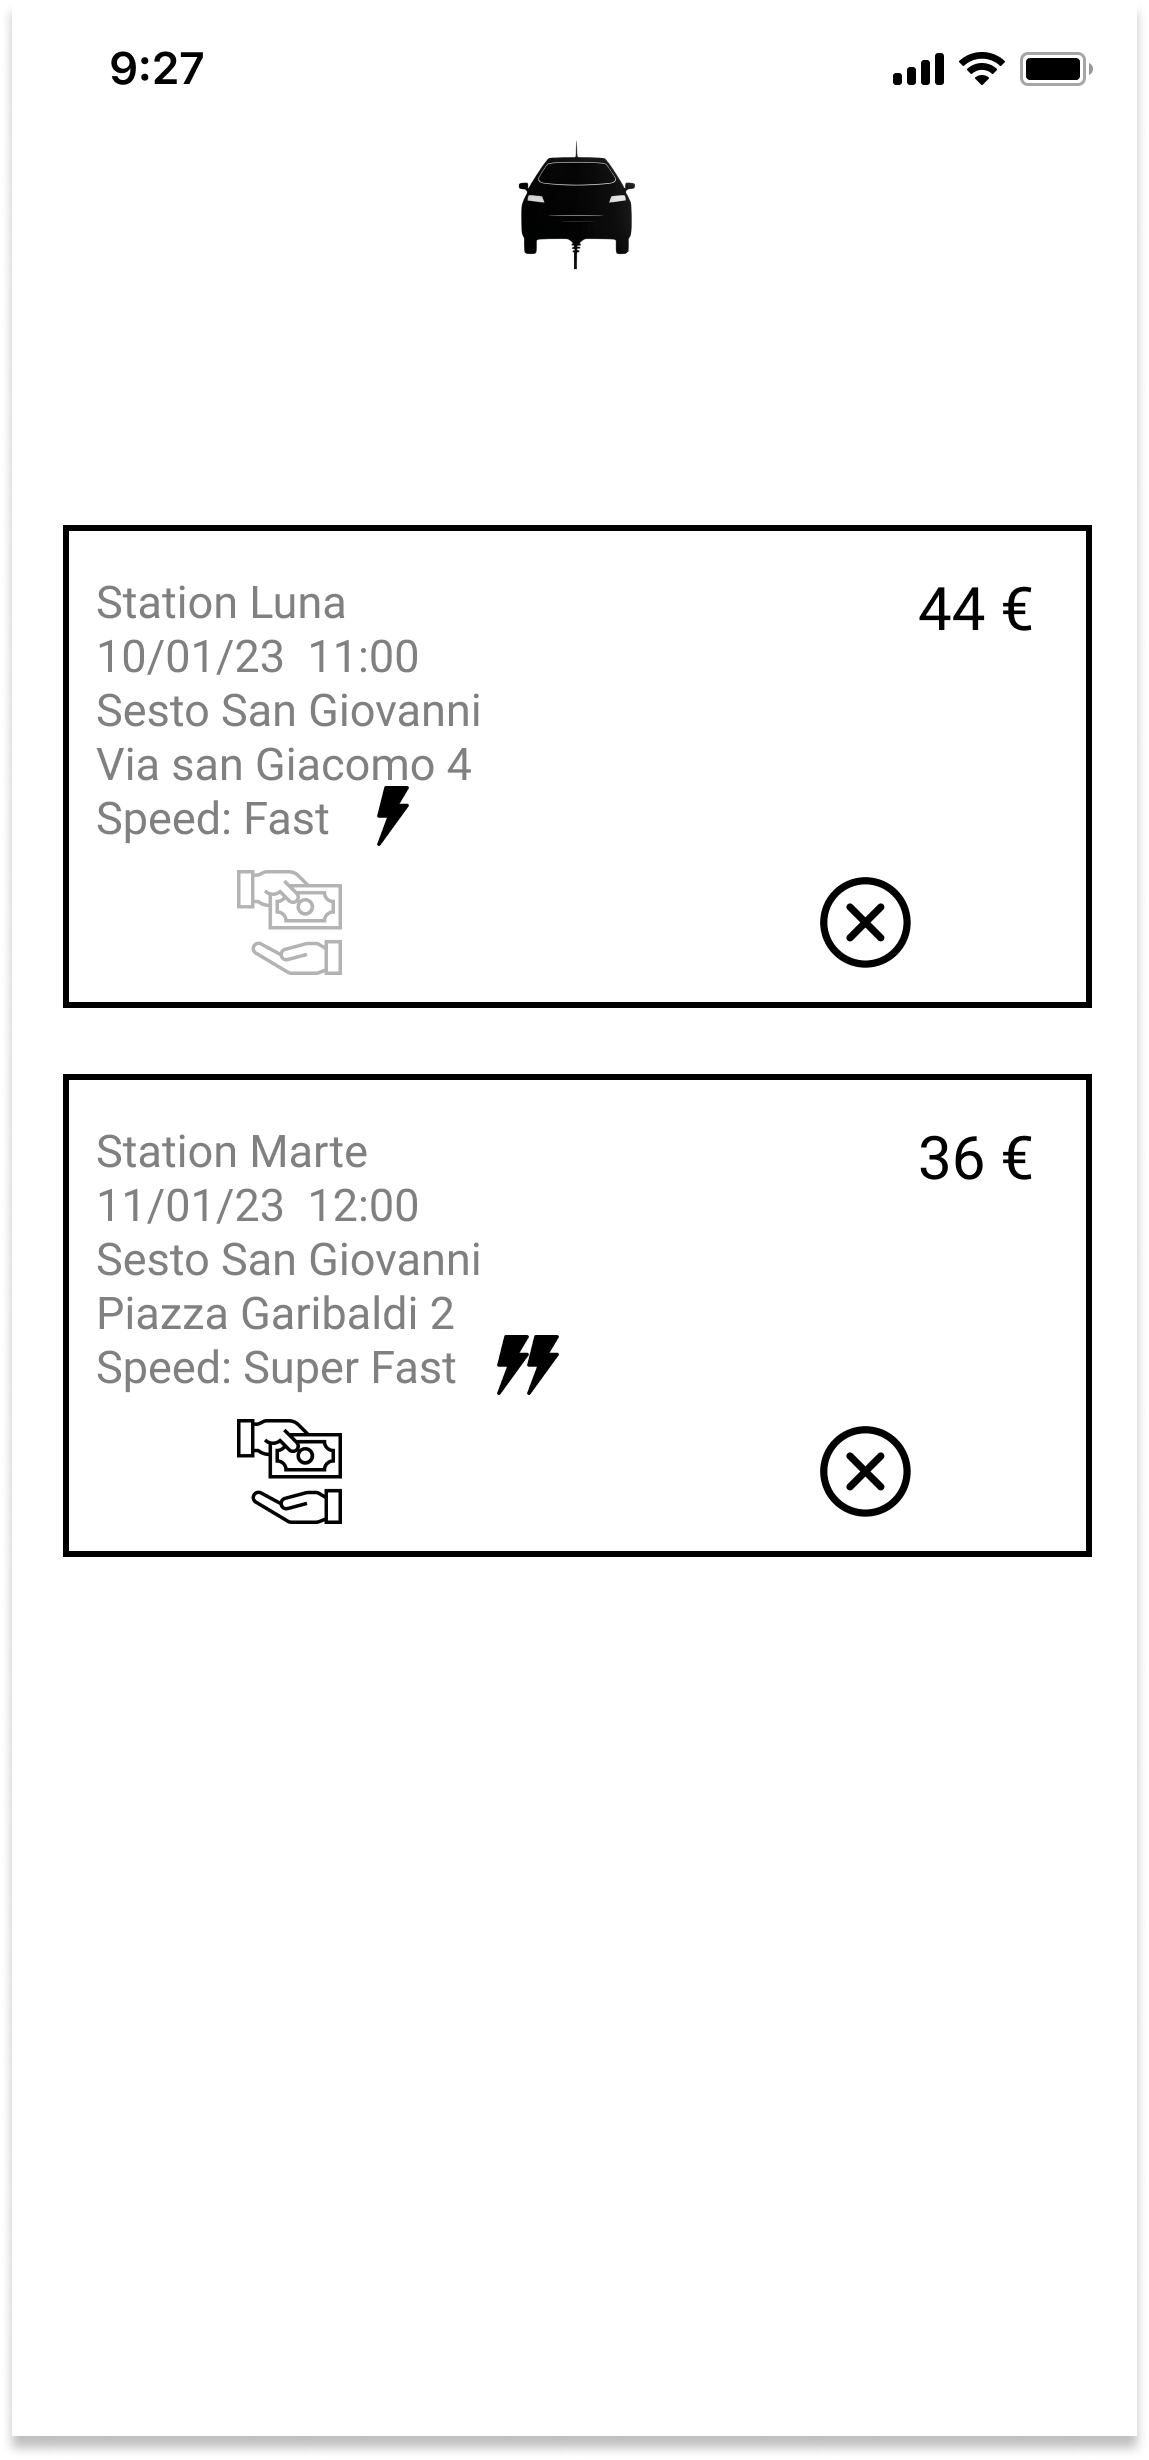
\includegraphics[keepaspectratio, height=15cm]{Mockup/UserAppInterface/My Charges.png}
    \caption{User Manages Charges}
    \label{fig:myCharges}
\end{figure}
In this section the user can see a list his/hers booked charges; for each booking the name, date, time frame and charge speed are displayed; the user can also pay for the charge by pressing the pay button and opening the \hyperref[pop:Pay]{pay popup} and delete a charge by pressing the delete button and opening the \hyperref[pop:Delete]{delete popup}. The charge has been already paid (cannot be paid again) if the pay button is greyed out.\\
By pressing the car logo the user can switch his/hers view to the \hyperref[fig:Search]{search page}.
\subsubsection{Pay a Charge}
\begin{figure}[H]
    \centering
    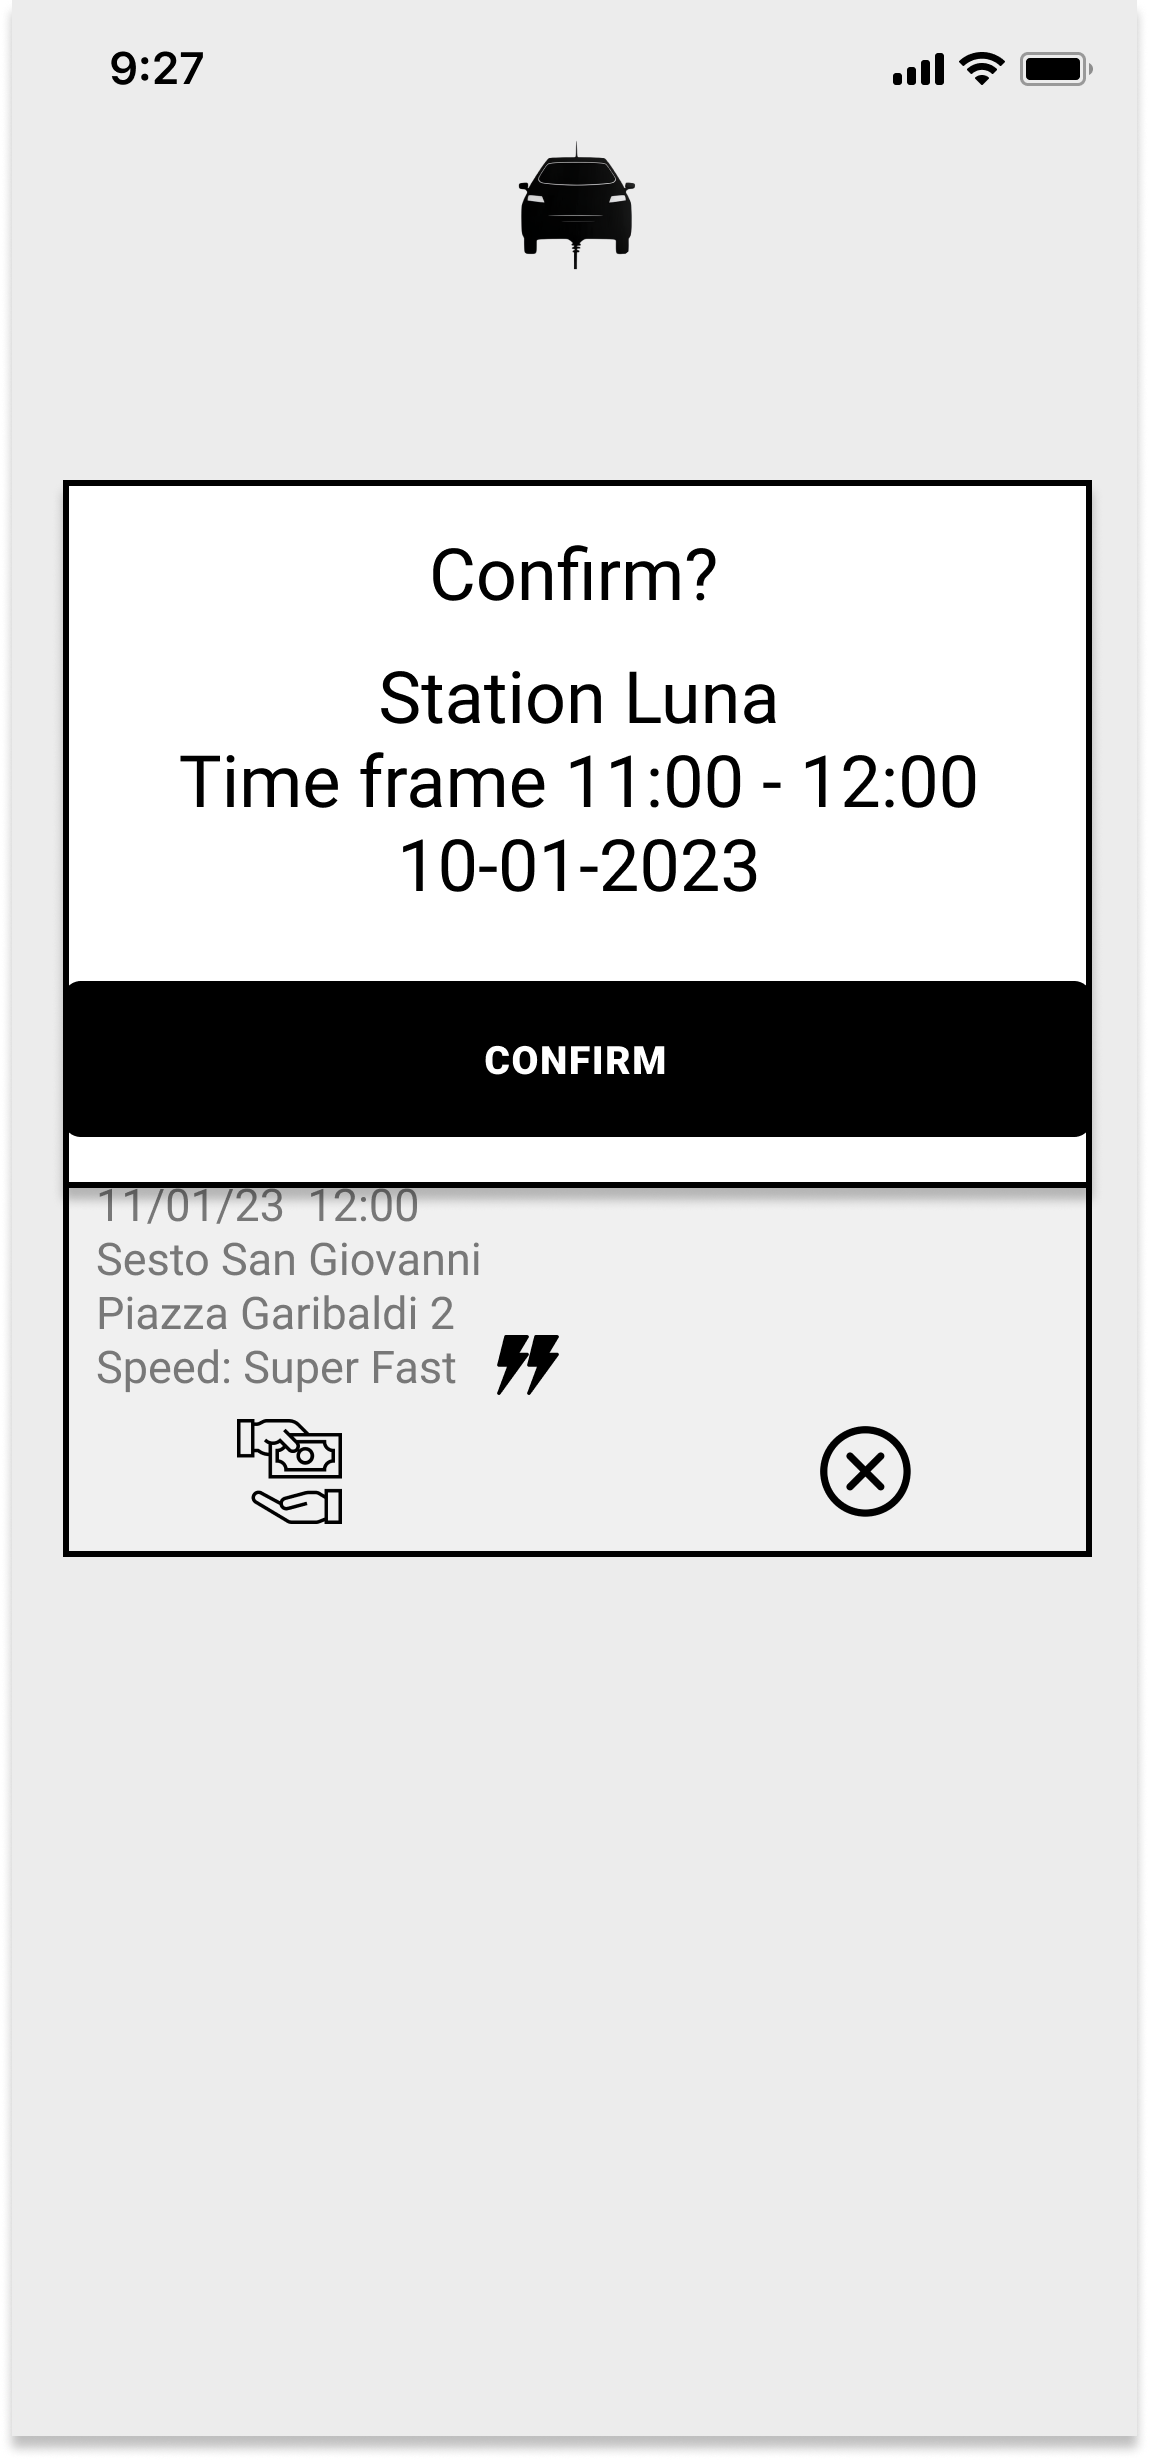
\includegraphics[keepaspectratio, height=15cm]{Mockup/UserAppInterface/Pay Charge.png}
    \caption{User Pay a Charge}
    \label{pop:Pay}
\end{figure}
In this section the detail of the charge are displayed and the user can pay the charge by pressing the confirm button.
\subsubsection{Cancel a Charge}
\begin{figure}[H]
    \centering
    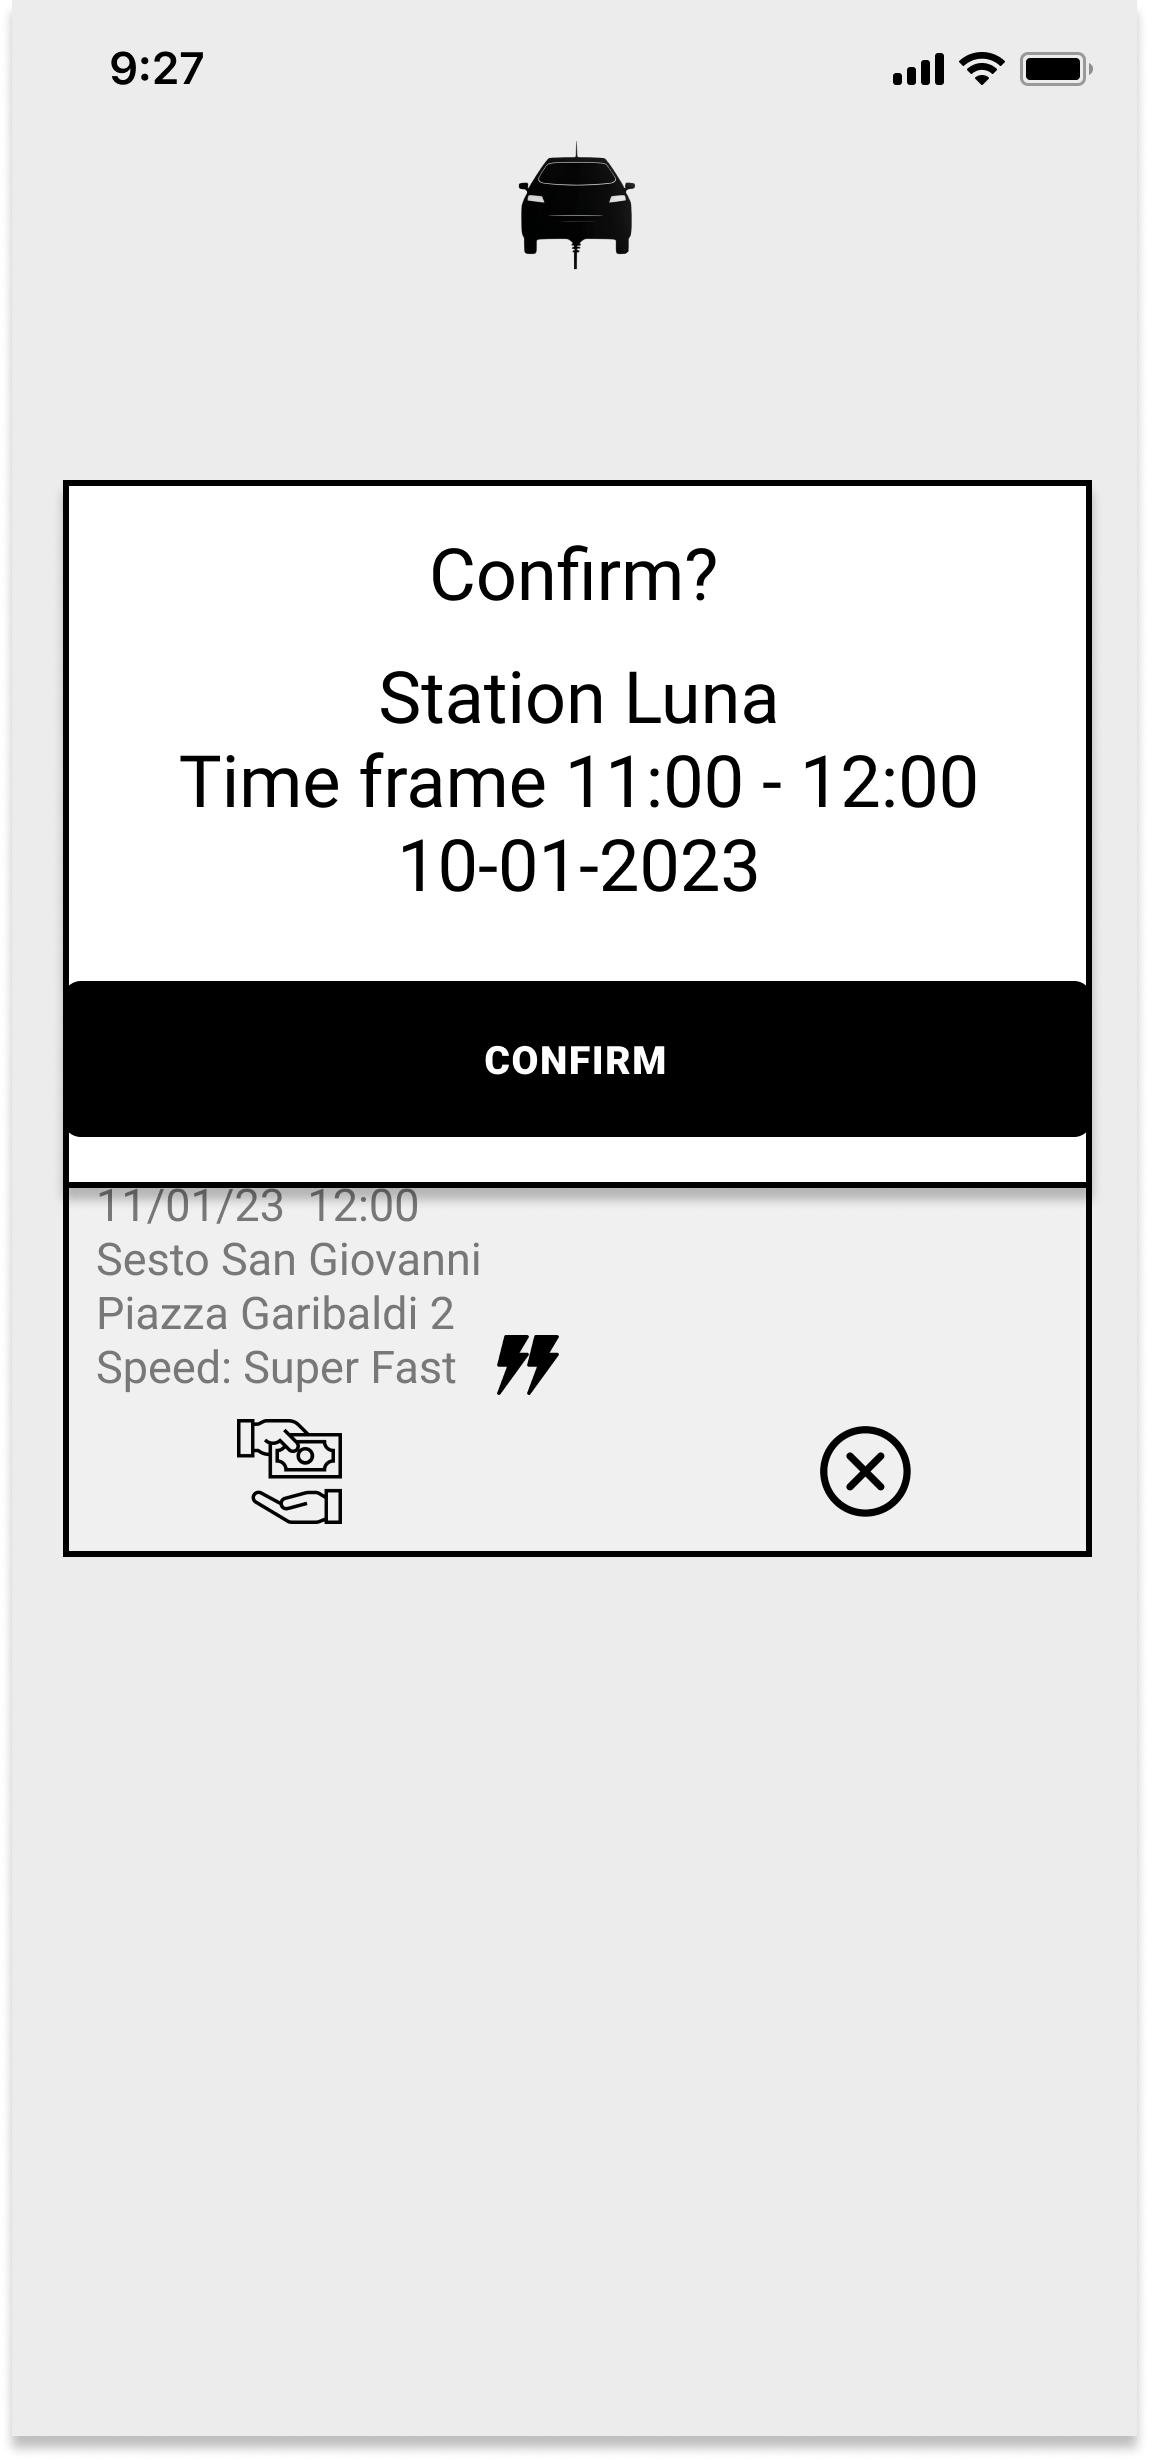
\includegraphics[keepaspectratio, height=15cm]{Mockup/UserAppInterface/Delete Charge.png}
    \caption{User Cancel a Charge}
    \label{pop:Delete}
\end{figure}
In this section the detail of the charge are displayed and the user can cancel the charge by pressing the confirm button.

\subsubsection{Suggest a charge}

\begin{figure}[H]
    \centering
    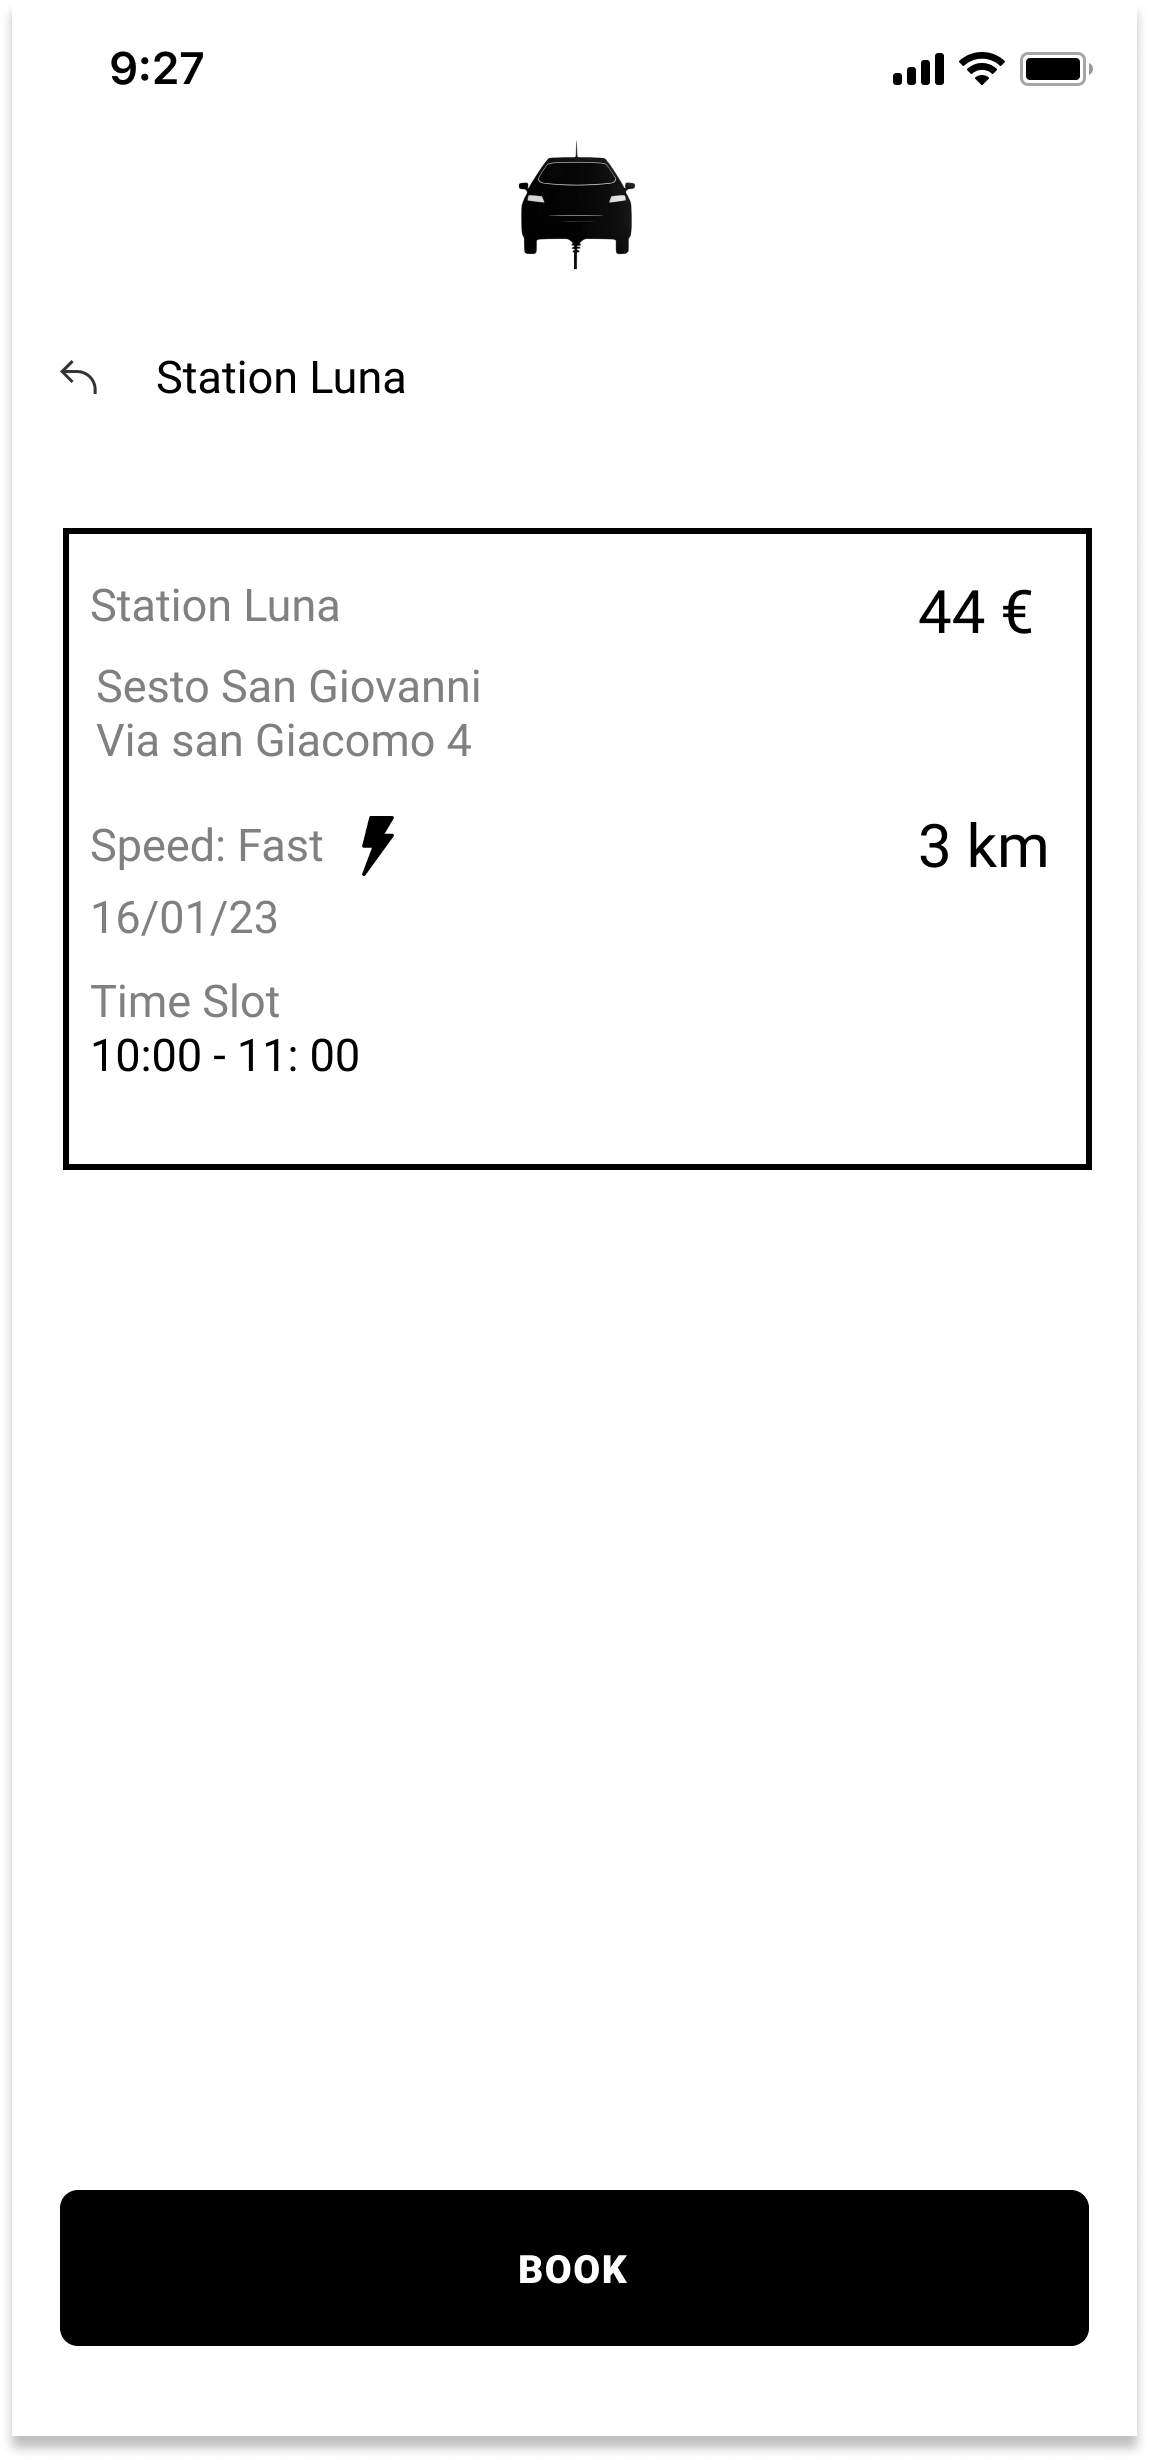
\includegraphics[keepaspectratio, height=15cm]{Mockup/UserAppInterface/Suggested Charge.png}
    \caption{User Gets Suggested Charge}
    \label{fig:Suggested}
\end{figure}
When the system think that a charge is needed/possible a notification to the user is sent, if the user opens it this page is displayed; here the info about the charge are shown and the booking can be confirmed by pressing the book button loading the \hyperref[pop:Booking]{booking popup}.\\
The user can return to the \hyperref[fig:Search]{search page} by pressing the backward arrow in the top left corner.
\subsection{CPO}
This section show the interface for the \ac{CPO}. The \ac{CPO} can do everything trough an app. The app is different than the one used by the user and it is assumed to be already installed on a device.
\subsubsection{Login}
\begin{figure}[H]
    \centering
    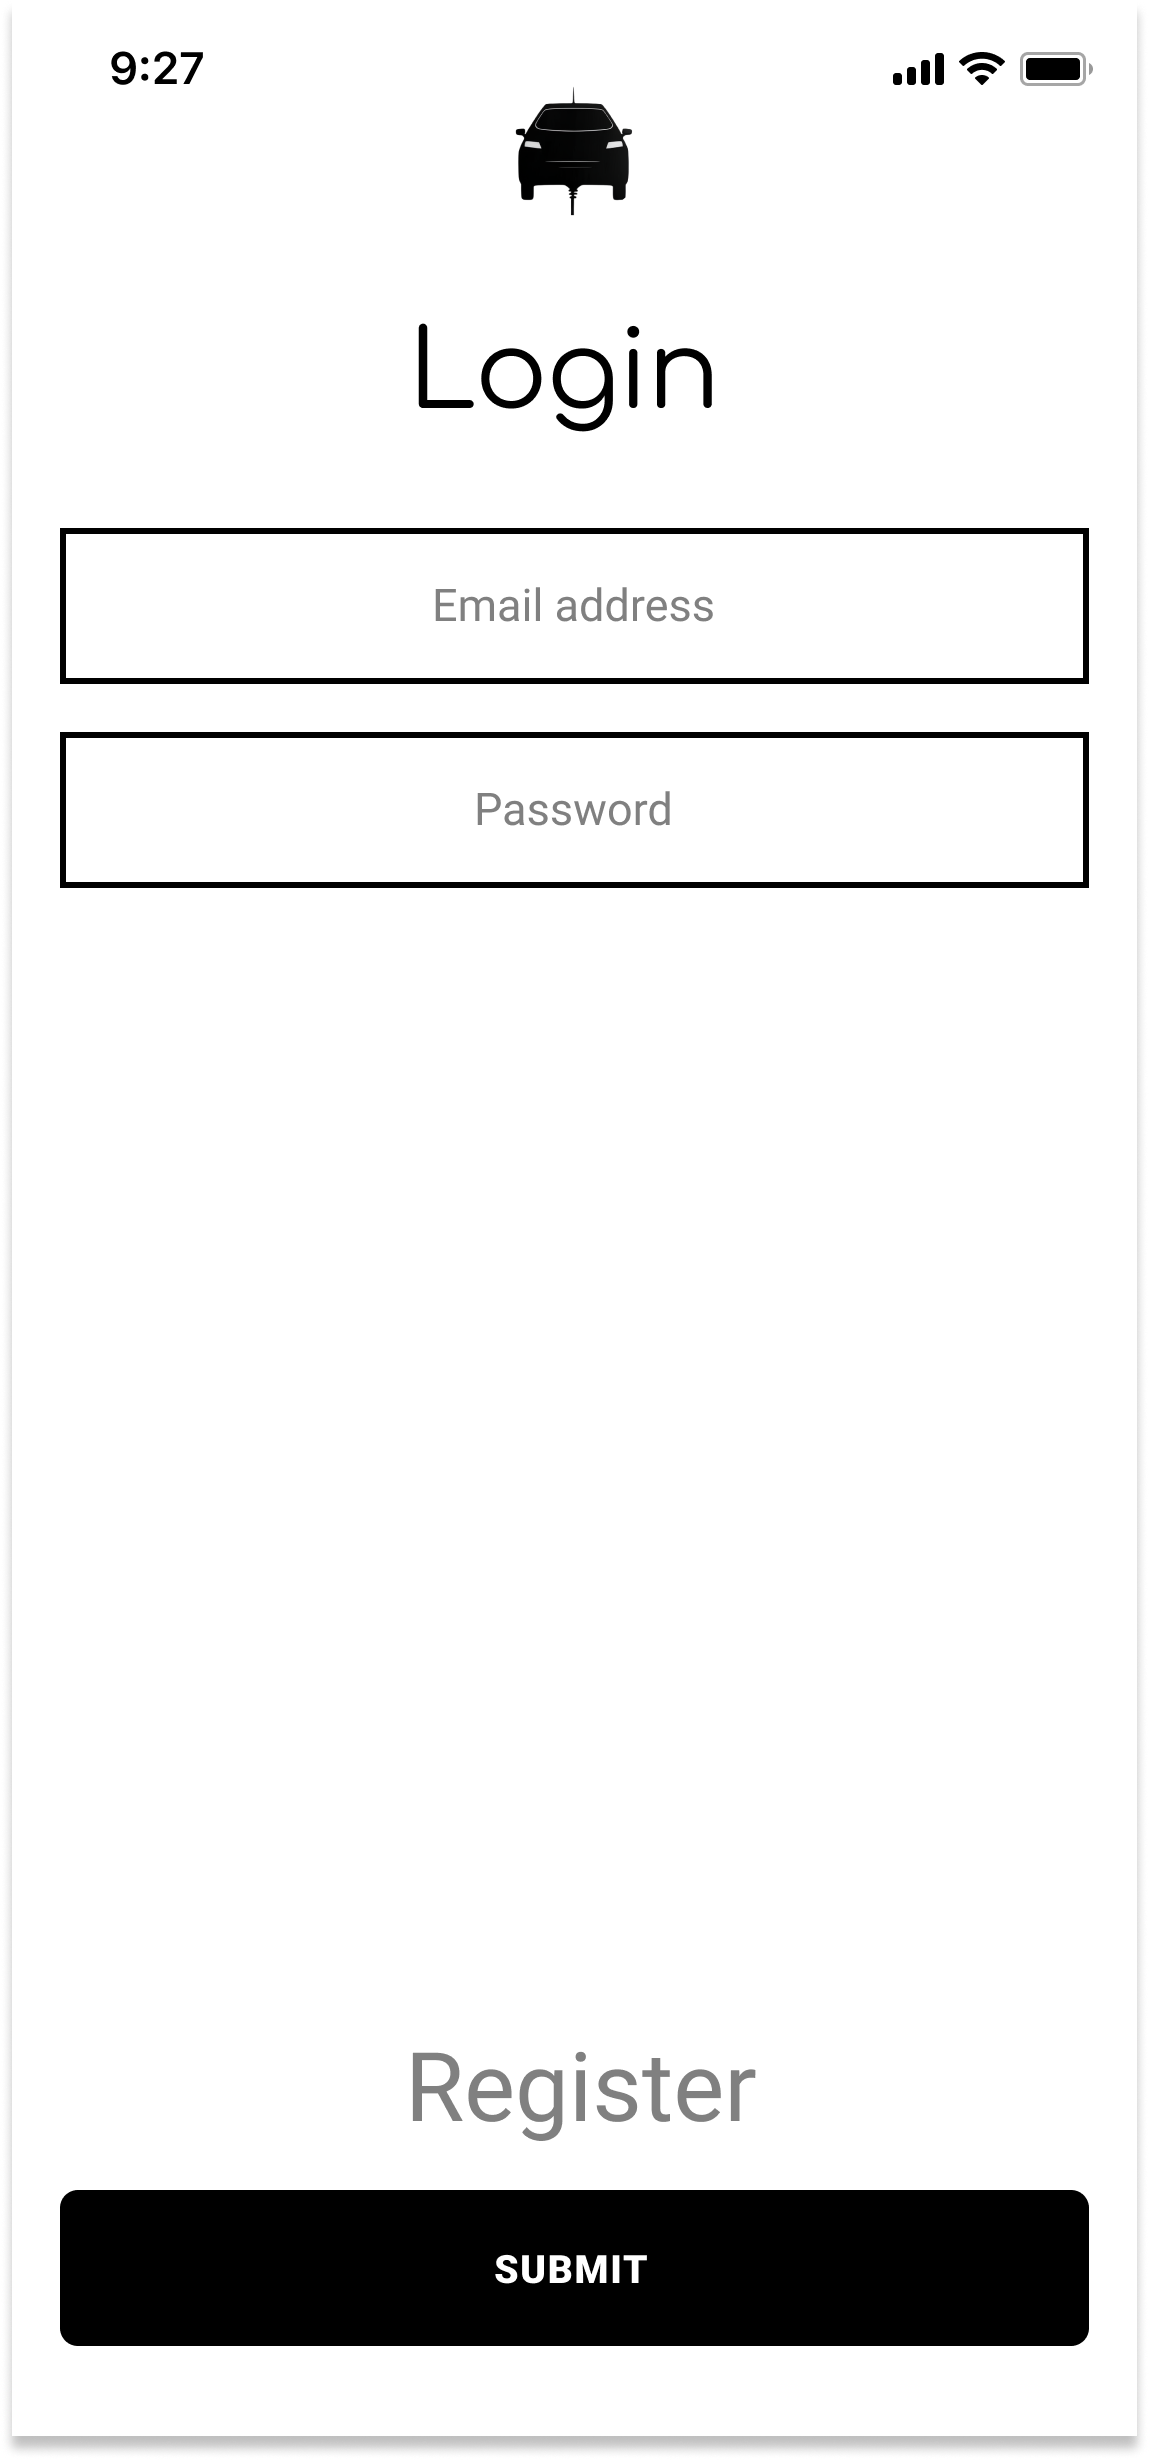
\includegraphics[keepaspectratio, height=15cm]{Mockup/CPOAppInterface/Login.png}
    \caption{\ac{CPO} Login}
    \label{site:Login}
\end{figure}
Once the \ac{CPO} opens the app this page is displayed. Here the \ac{CPO} can log into the system inserting the email and password provided during the registration. When the user press the submit button, if the information provided are correct, the \hyperref[site:Homepage]{homepage} is loaded,otherwise the \hyperref[site:FailedLogin]{failed login page} is shown.\\
The user can press the register button to open the \hyperref[fig:Register].\\
If the \ac{CPO} is not registered it can do it by pressing the Register button which loads the \hyperref[site:Register]{register page}.
{register page}.
\begin{figure}[H]
    \centering
    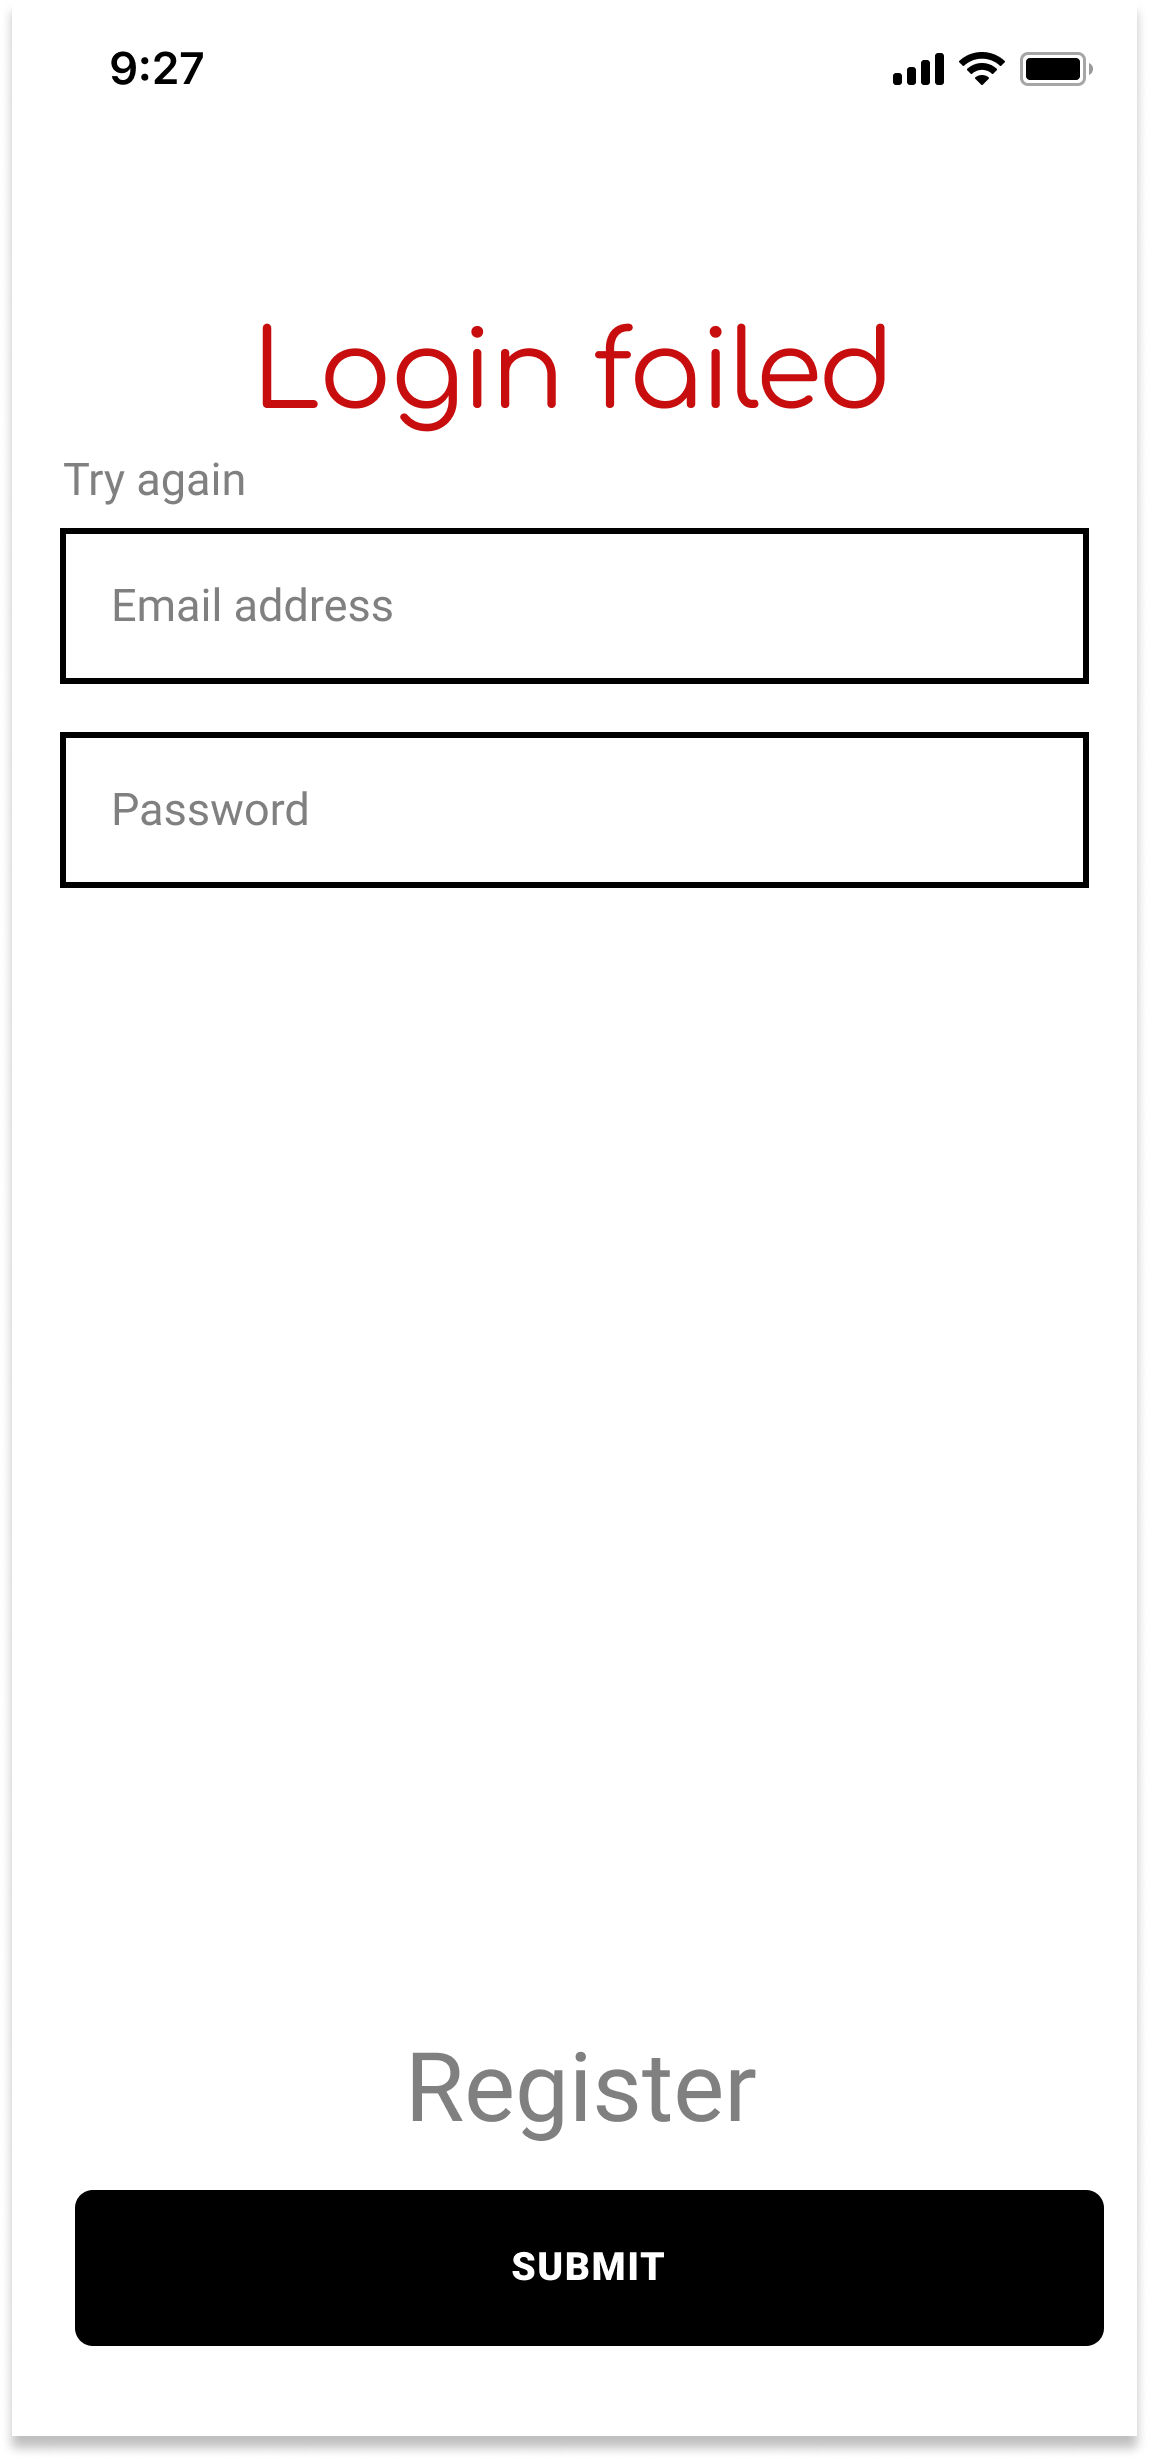
\includegraphics[keepaspectratio, height=15cm]{Mockup/CPOAppInterface/Failed Login.png}
    \caption{Wrong Credential}
    \label{site:FailedLogin}
\end{figure}
If the user has inserted the wrong email or password he/she can retry it in this page, otherwise the user can press the Sign Up button to open the \hyperref[site:Register]{register page}.
\subsubsection{Register}
\begin{figure}[H]
    \centering
    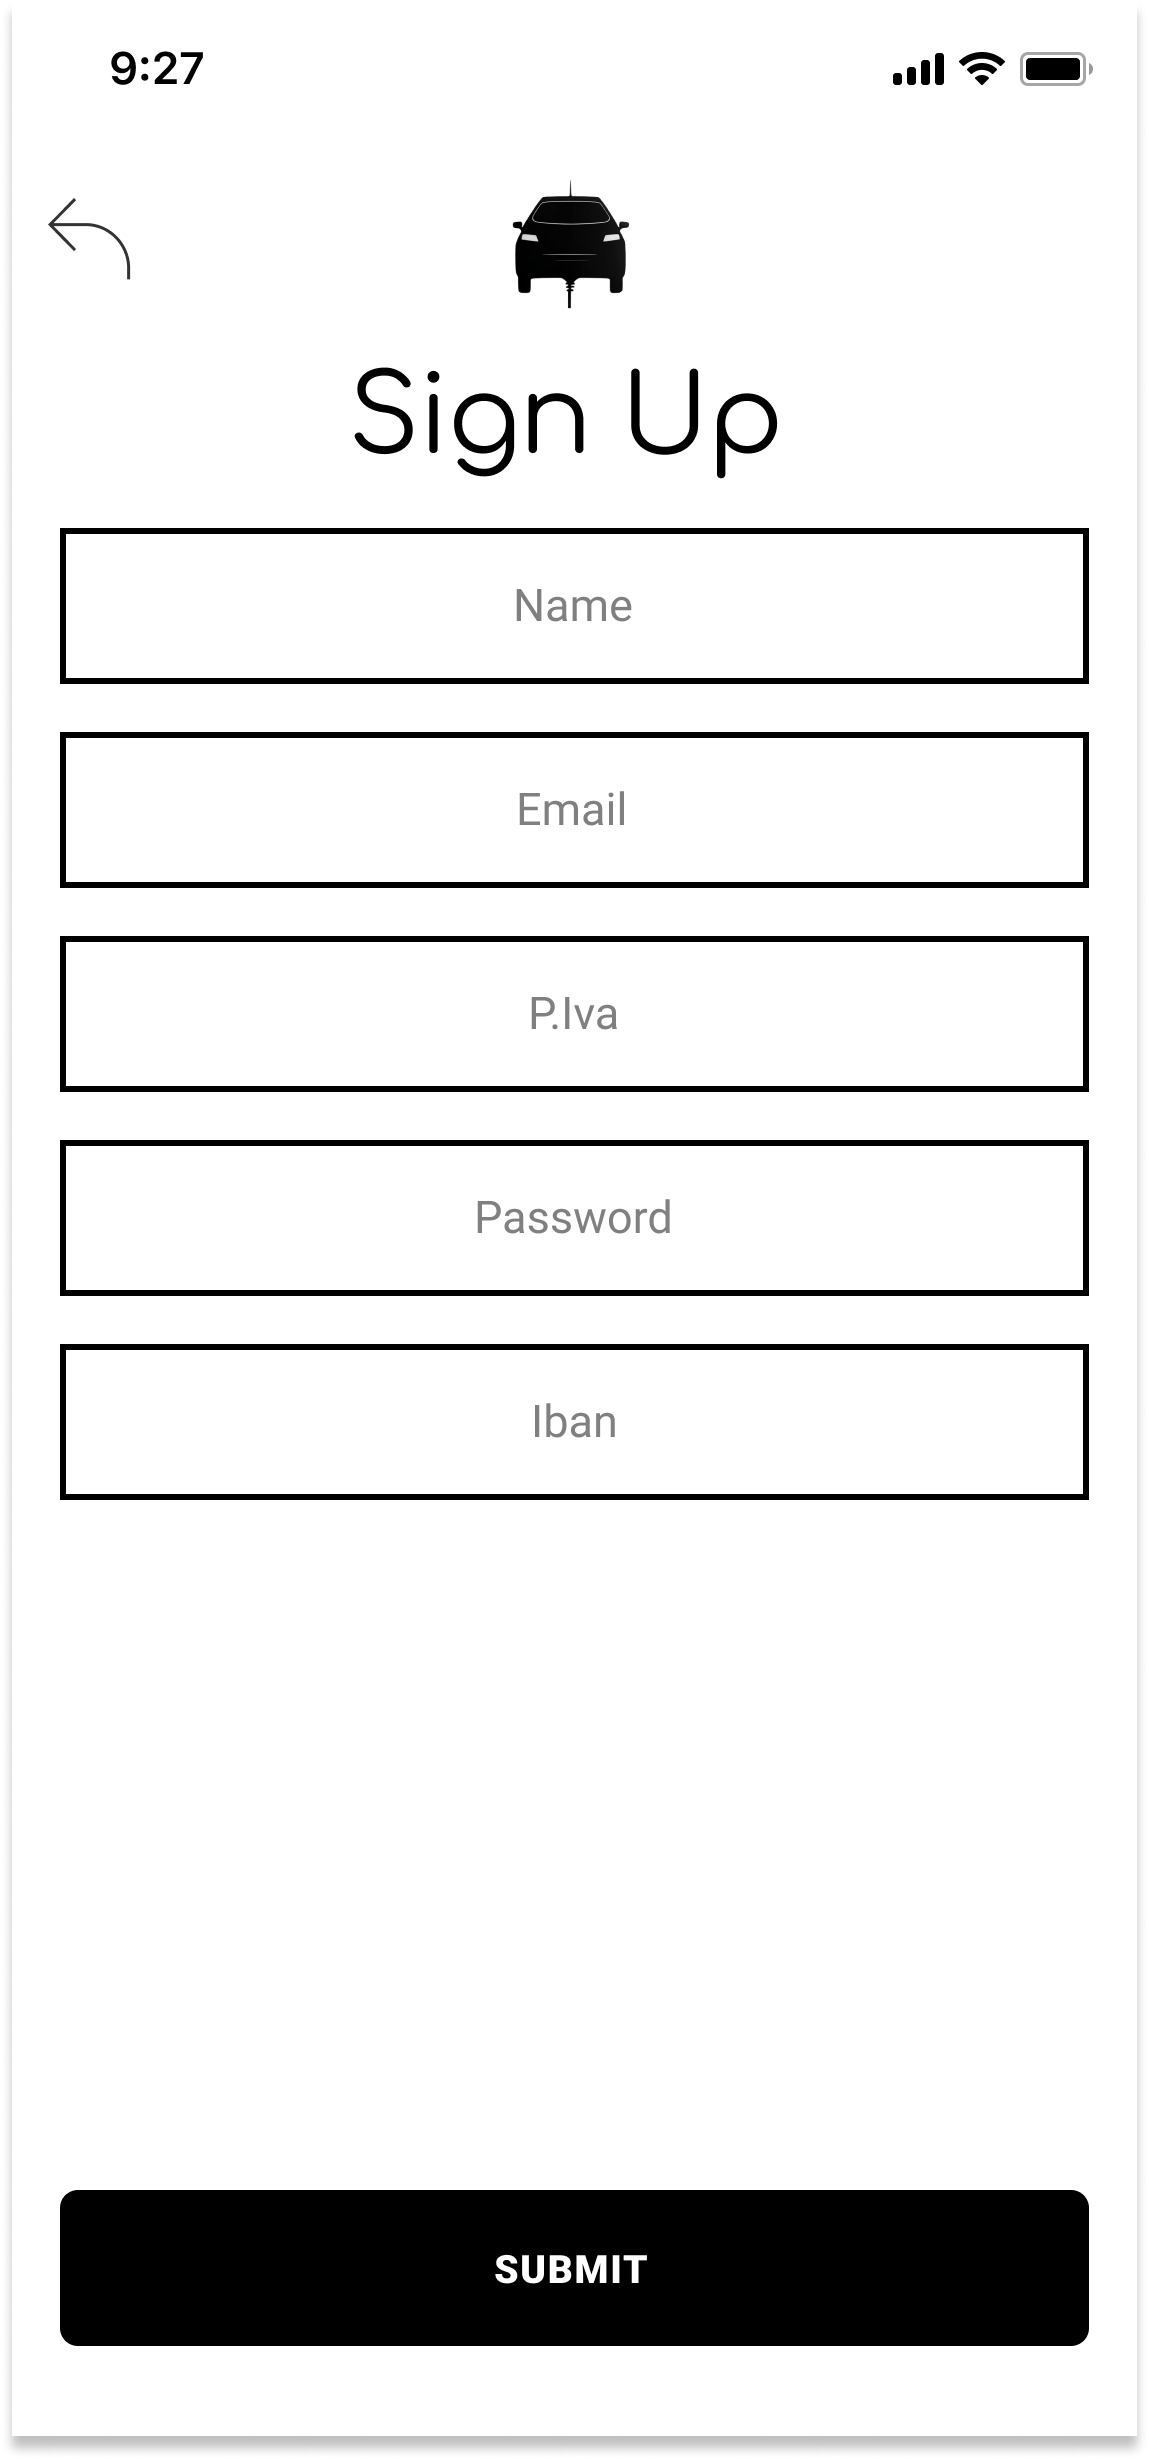
\includegraphics[keepaspectratio, height=15cm]{Mockup/CPOAppInterface/Register.png}
    \caption{\ac{CPO} Register}
    \label{site:Register}
\end{figure}
In this page the \ac{CPO} can register itself to the service by providing the asked information and pressing the submit. An email will be sent to the user with a link within, clicking the link will open the app displaying the \hyperref[site:ConfirmReg]{confirmation page} completing the registration procedure.\\
If the user wants to return to the \hyperref[fig:Login]{login page} he can do so by pressing the backward arrow in the top left corner.
\begin{figure}[H]
    \centering
    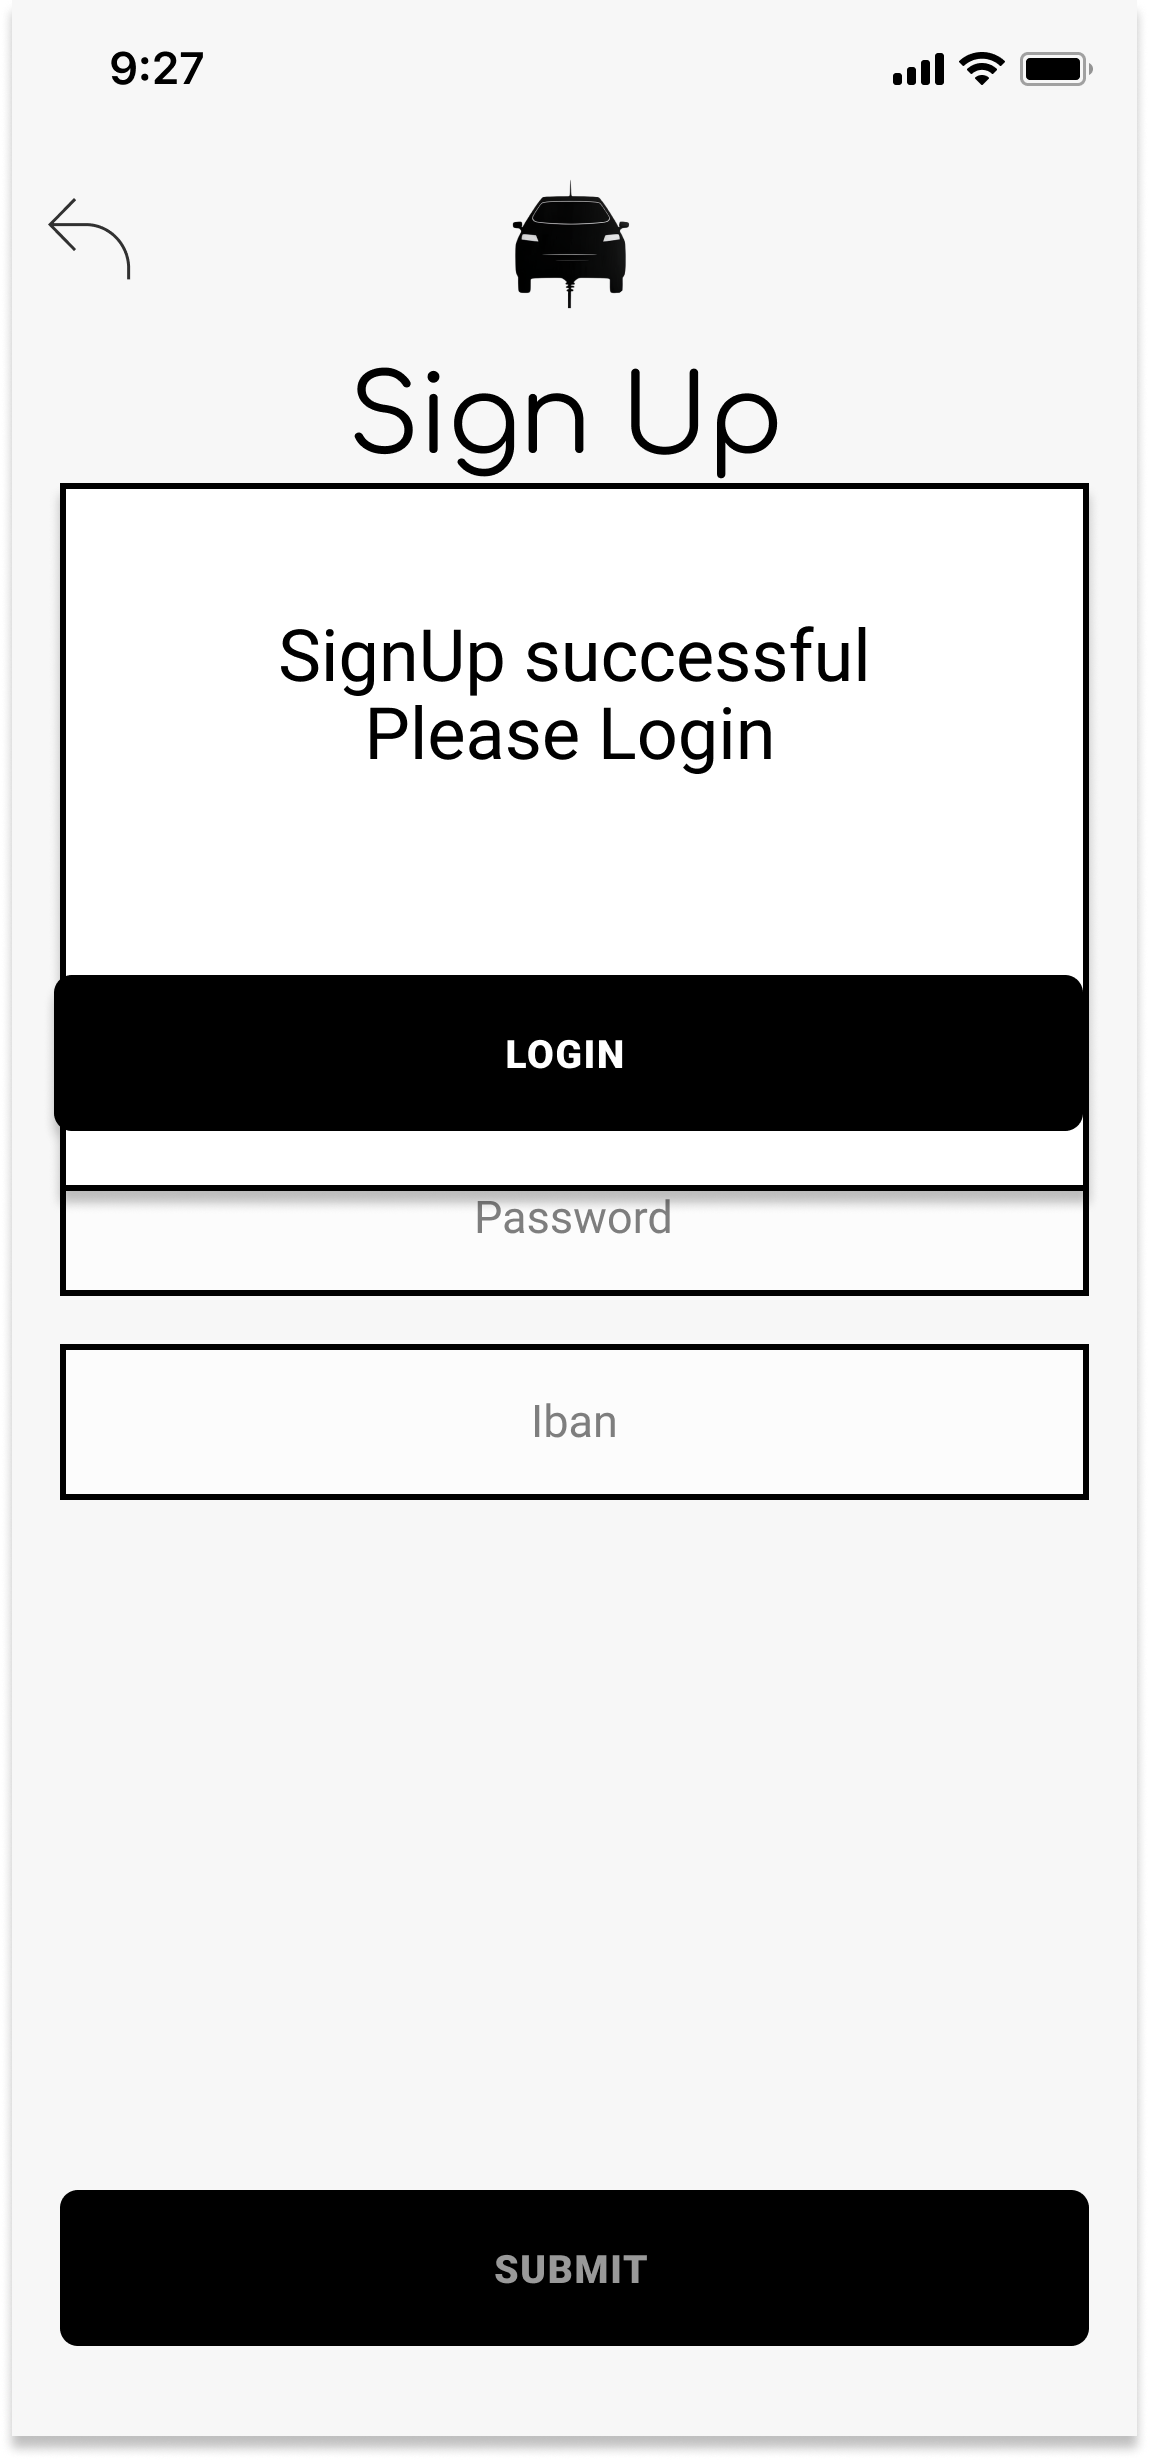
\includegraphics[keepaspectratio, height=15cm]{Mockup/CPOAppInterface/RegisterConfirmation.png}
    \caption{User Finish Registering}
    \label{site:ConfirmReg}
\end{figure}
once this page is displayed the user has to log in by clicking the log in button which opens the \hyperref[site:Login]{login page}.
\subsubsection{Home Page}
\begin{figure}[H]
    \centering
    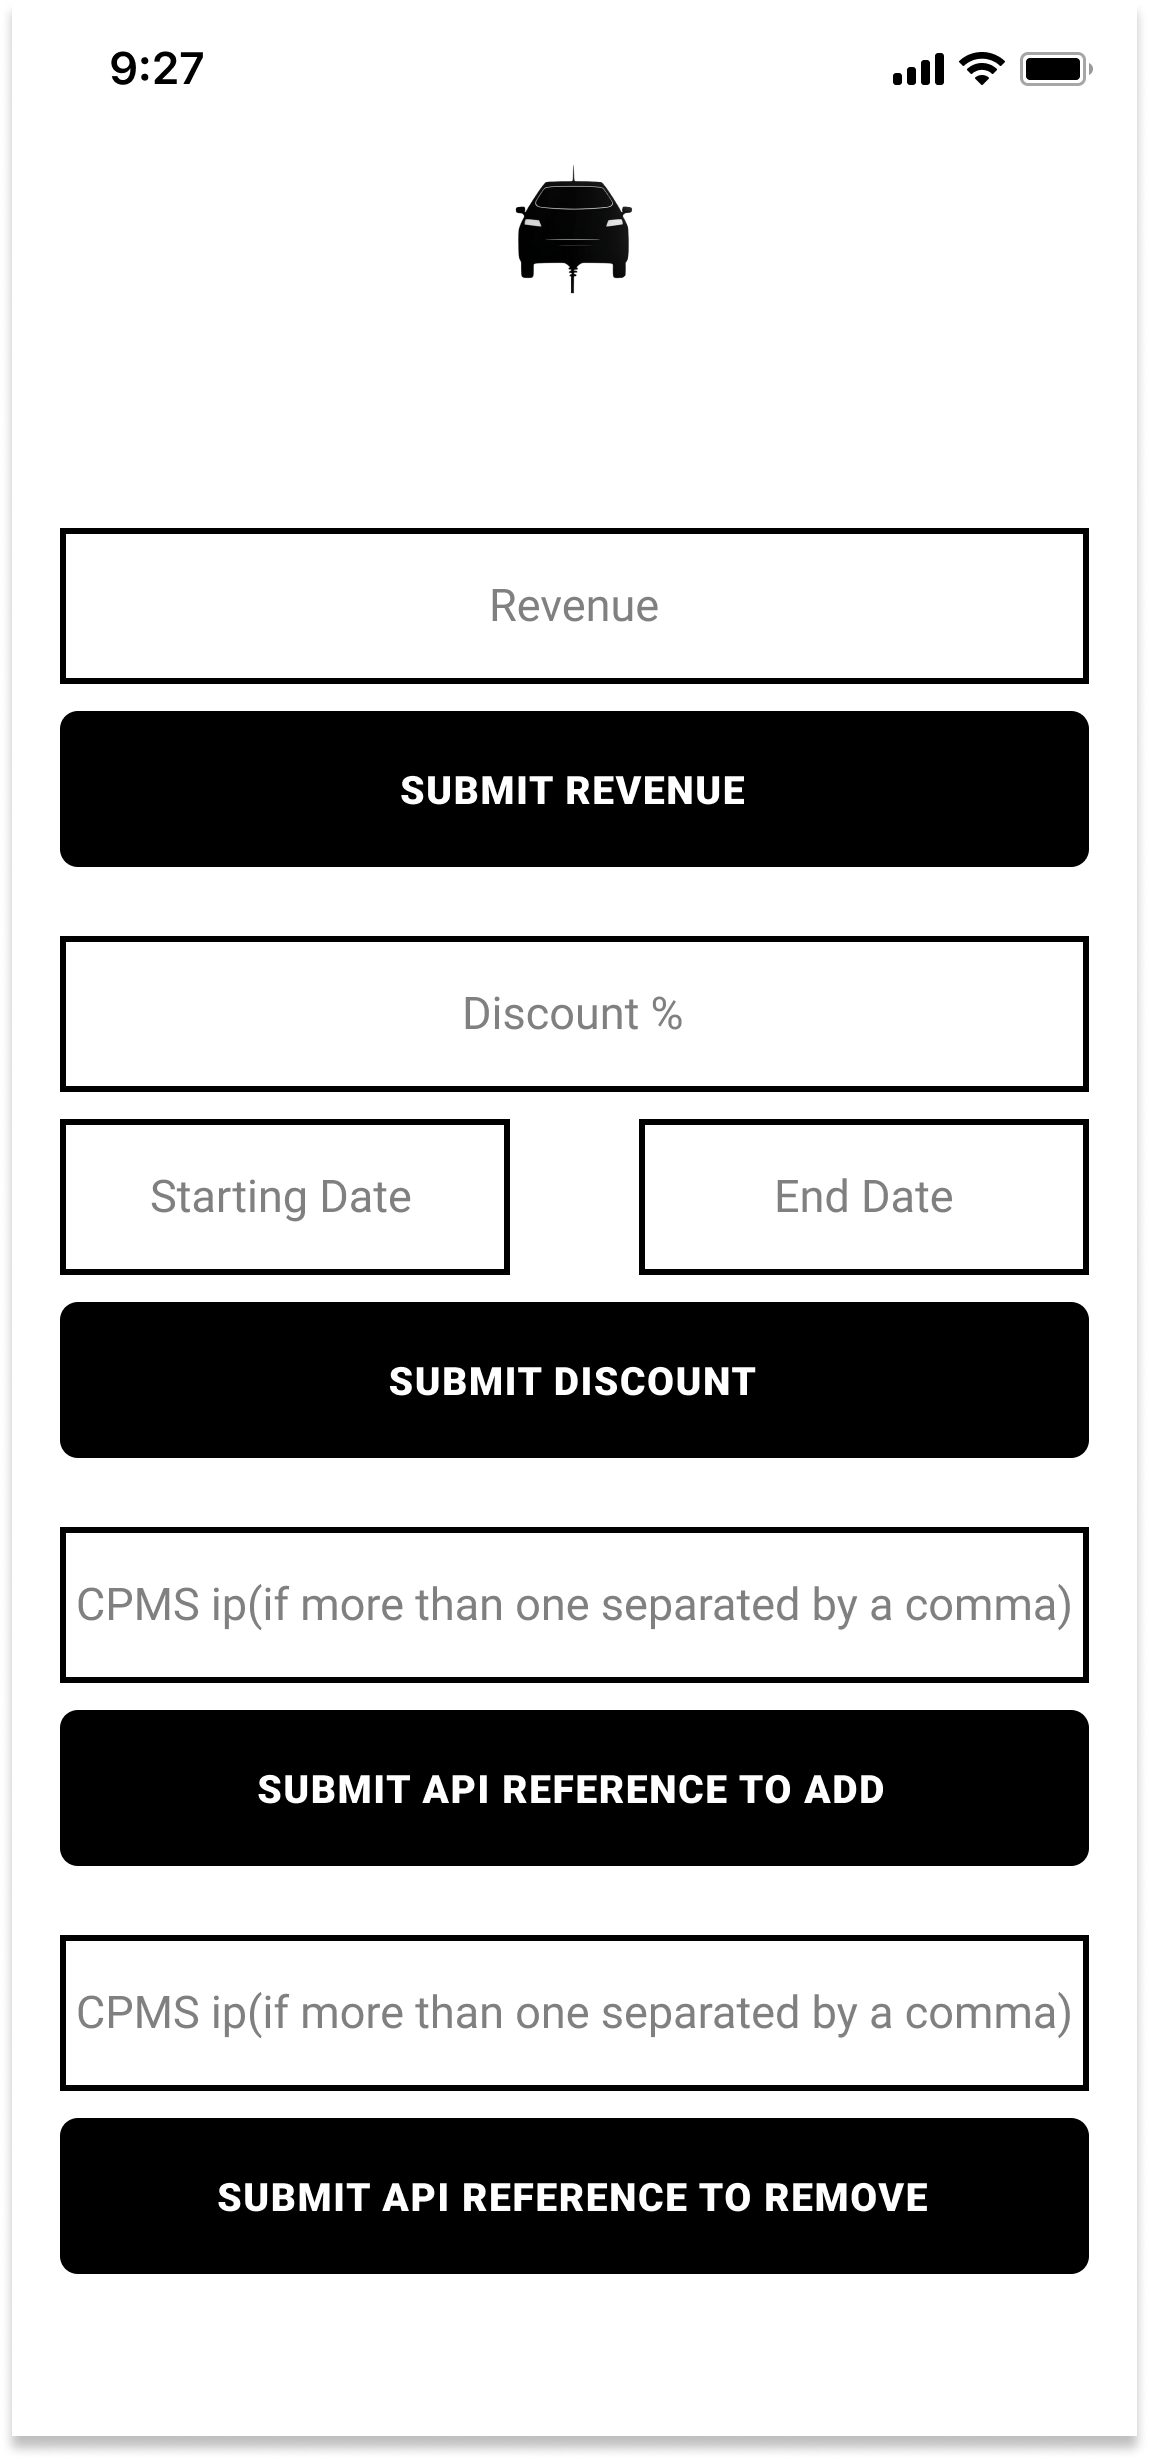
\includegraphics[keepaspectratio, height=15cm]{Mockup/CPOAppInterface/Homepage.png}
    \caption{\ac{CPO} access the site functions}
    \label{site:Homepage}
\end{figure}
In this page the \ac{CPO} can change the revenue, create discounts and add cpms reference.
To change the Revenue the user has to insert the new revenue percentage in the field and press the submit revenue button, the revenue will be updated and the page refreshed.\\
To create new discounts the user hast to insert the percentage of discounts, the time frame of the discount and press the submit discount button, the discount will be updated and the page refreshed.\\
To add new Cpms the user has to insert the IP to the \ac{CPMS} ( if more than one separated by a comma) and press the submit \ac{API} reference to add button, the \ac{API} reference will be updated and the page refreshed.\\
To remove a Cpms the user has to insert the IP to the \ac{CPMS} ( if more than one separated by a comma) and press the submit \ac{API} reference to remove button, the \ac{CPMS} will be removed and the page refreshed.

\subsection{CPOMaintainer}
This are the interfaces for the maintainers to access their \acp{CPMS}, it is assumed that the maintainer is already connected to the \ac{VPN} trough a pc and a internet connection.
\subsubsection{Login}
\begin{figure}[H]
    \centering
    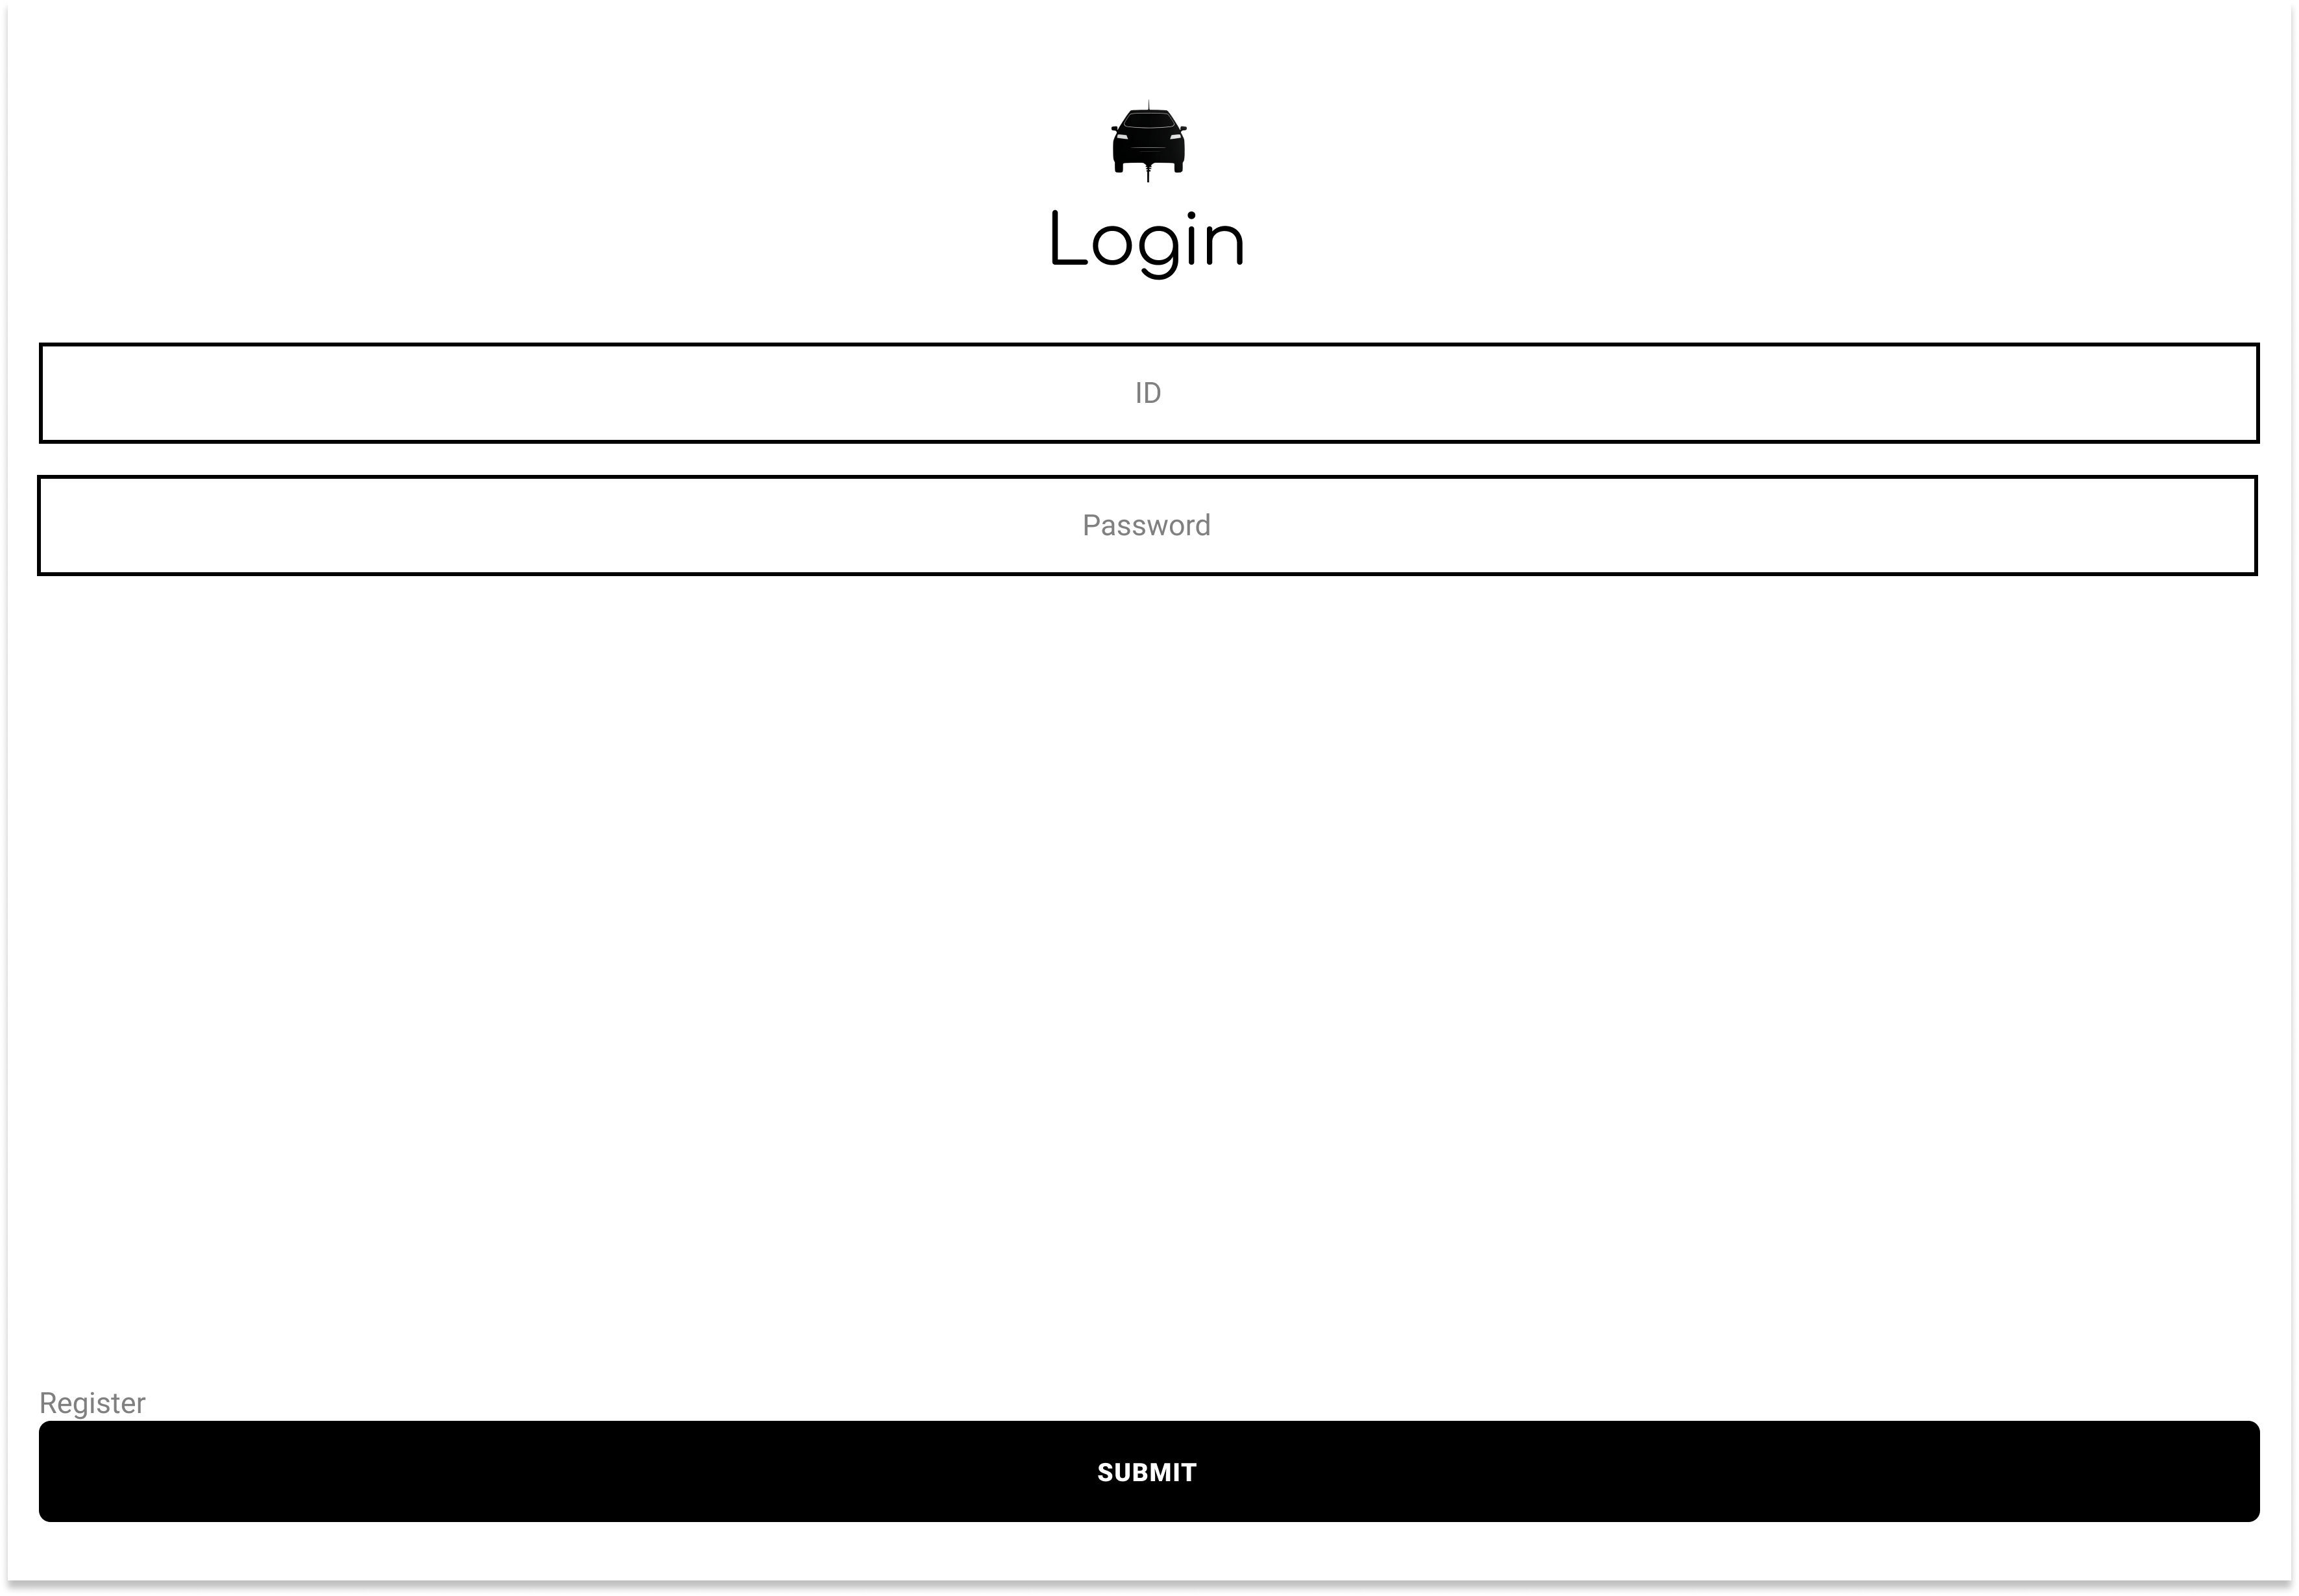
\includegraphics[keepaspectratio, width=15cm]{Mockup/CPMSSiteInterface/Login.png}
    \caption{\ac{CPO}Maintainer logs In}
    \label{cpo:Login}
\end{figure}
Here the \ac{CPO}Maintainer can access the \ac{CPMS} by inserting the correct ID and password and pressing the submit button. If the data is valid the \hyperref[cpo:Homepage]{homepage} is displayed.
\subsubsection{Homepage}
\begin{figure}[H]
    \centering
    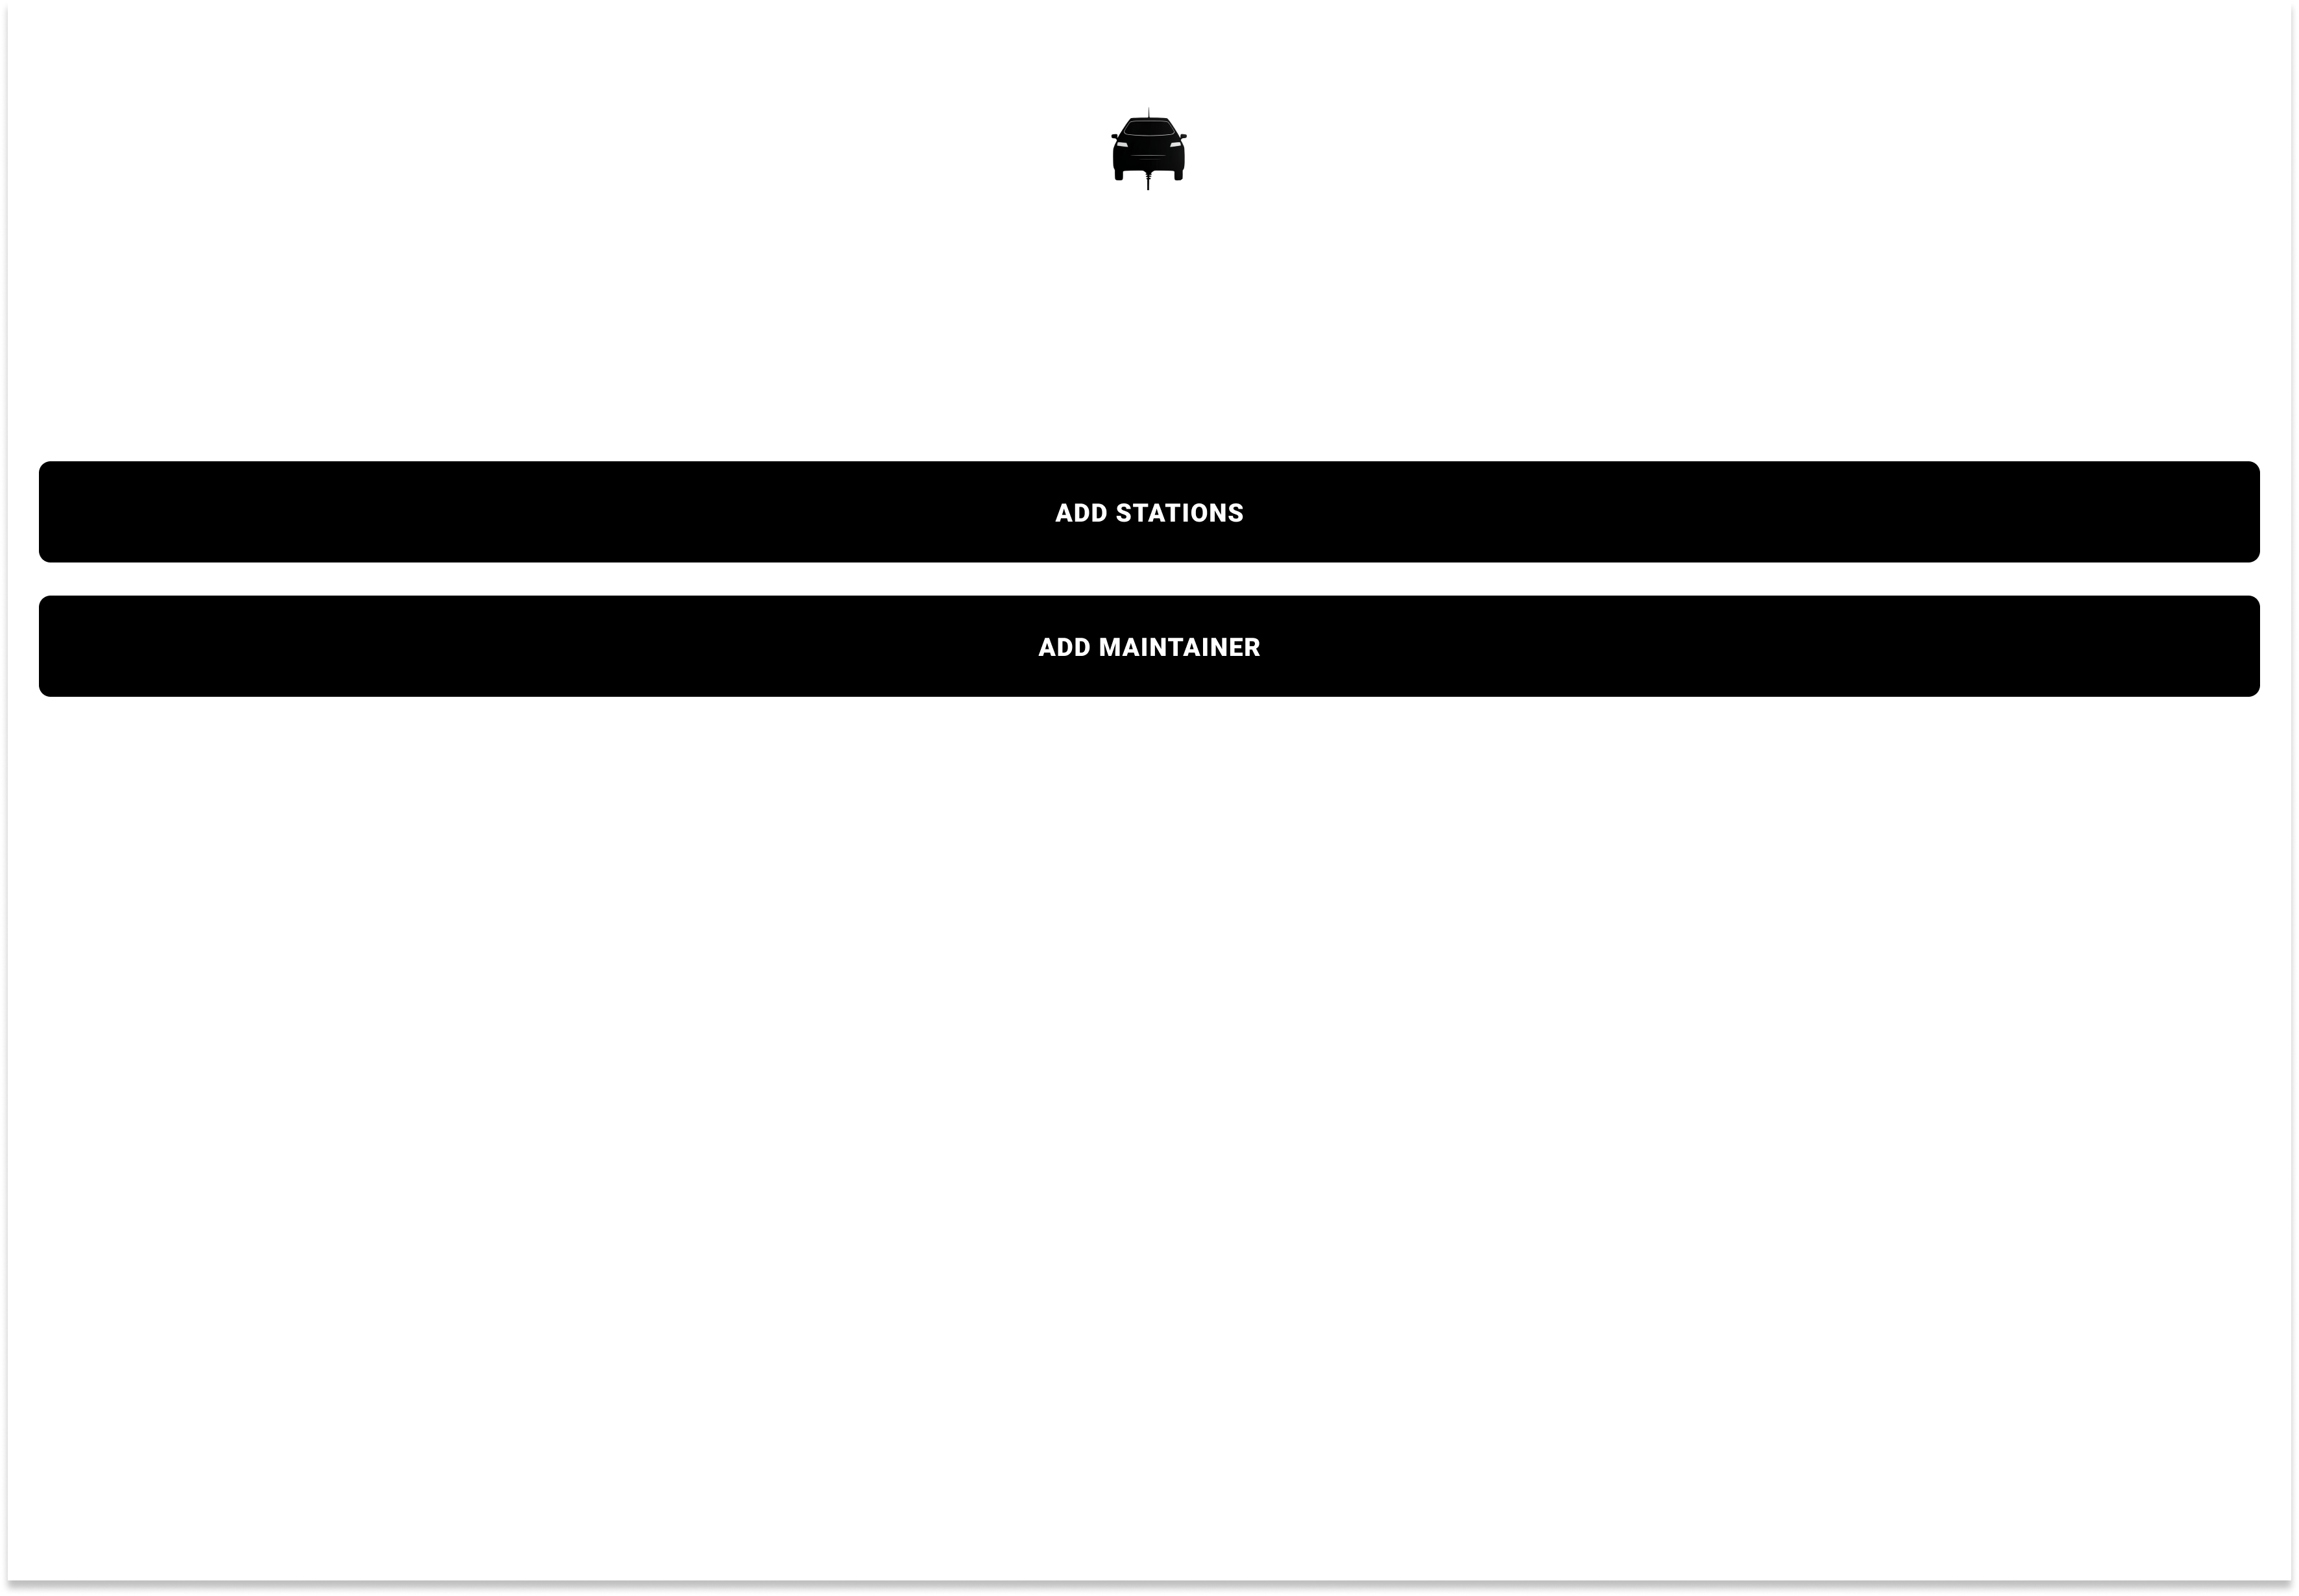
\includegraphics[keepaspectratio, width=15cm]{Mockup/CPMSSiteInterface/Homepage.png}
    \caption{\ac{CPO} access the site functions}
    \label{cpo:Homepage}
    Here the maintainer can select the function to operate by either clicking the add station button (opening the \hyperref[cpo:Station]{add station page}) or clicking the add maintainer button (opening the \hyperref[cpo:Maintainer]{add maintainer page})
\end{figure}
\subsubsection{Station Management}
\begin{figure}[H]
    \centering
    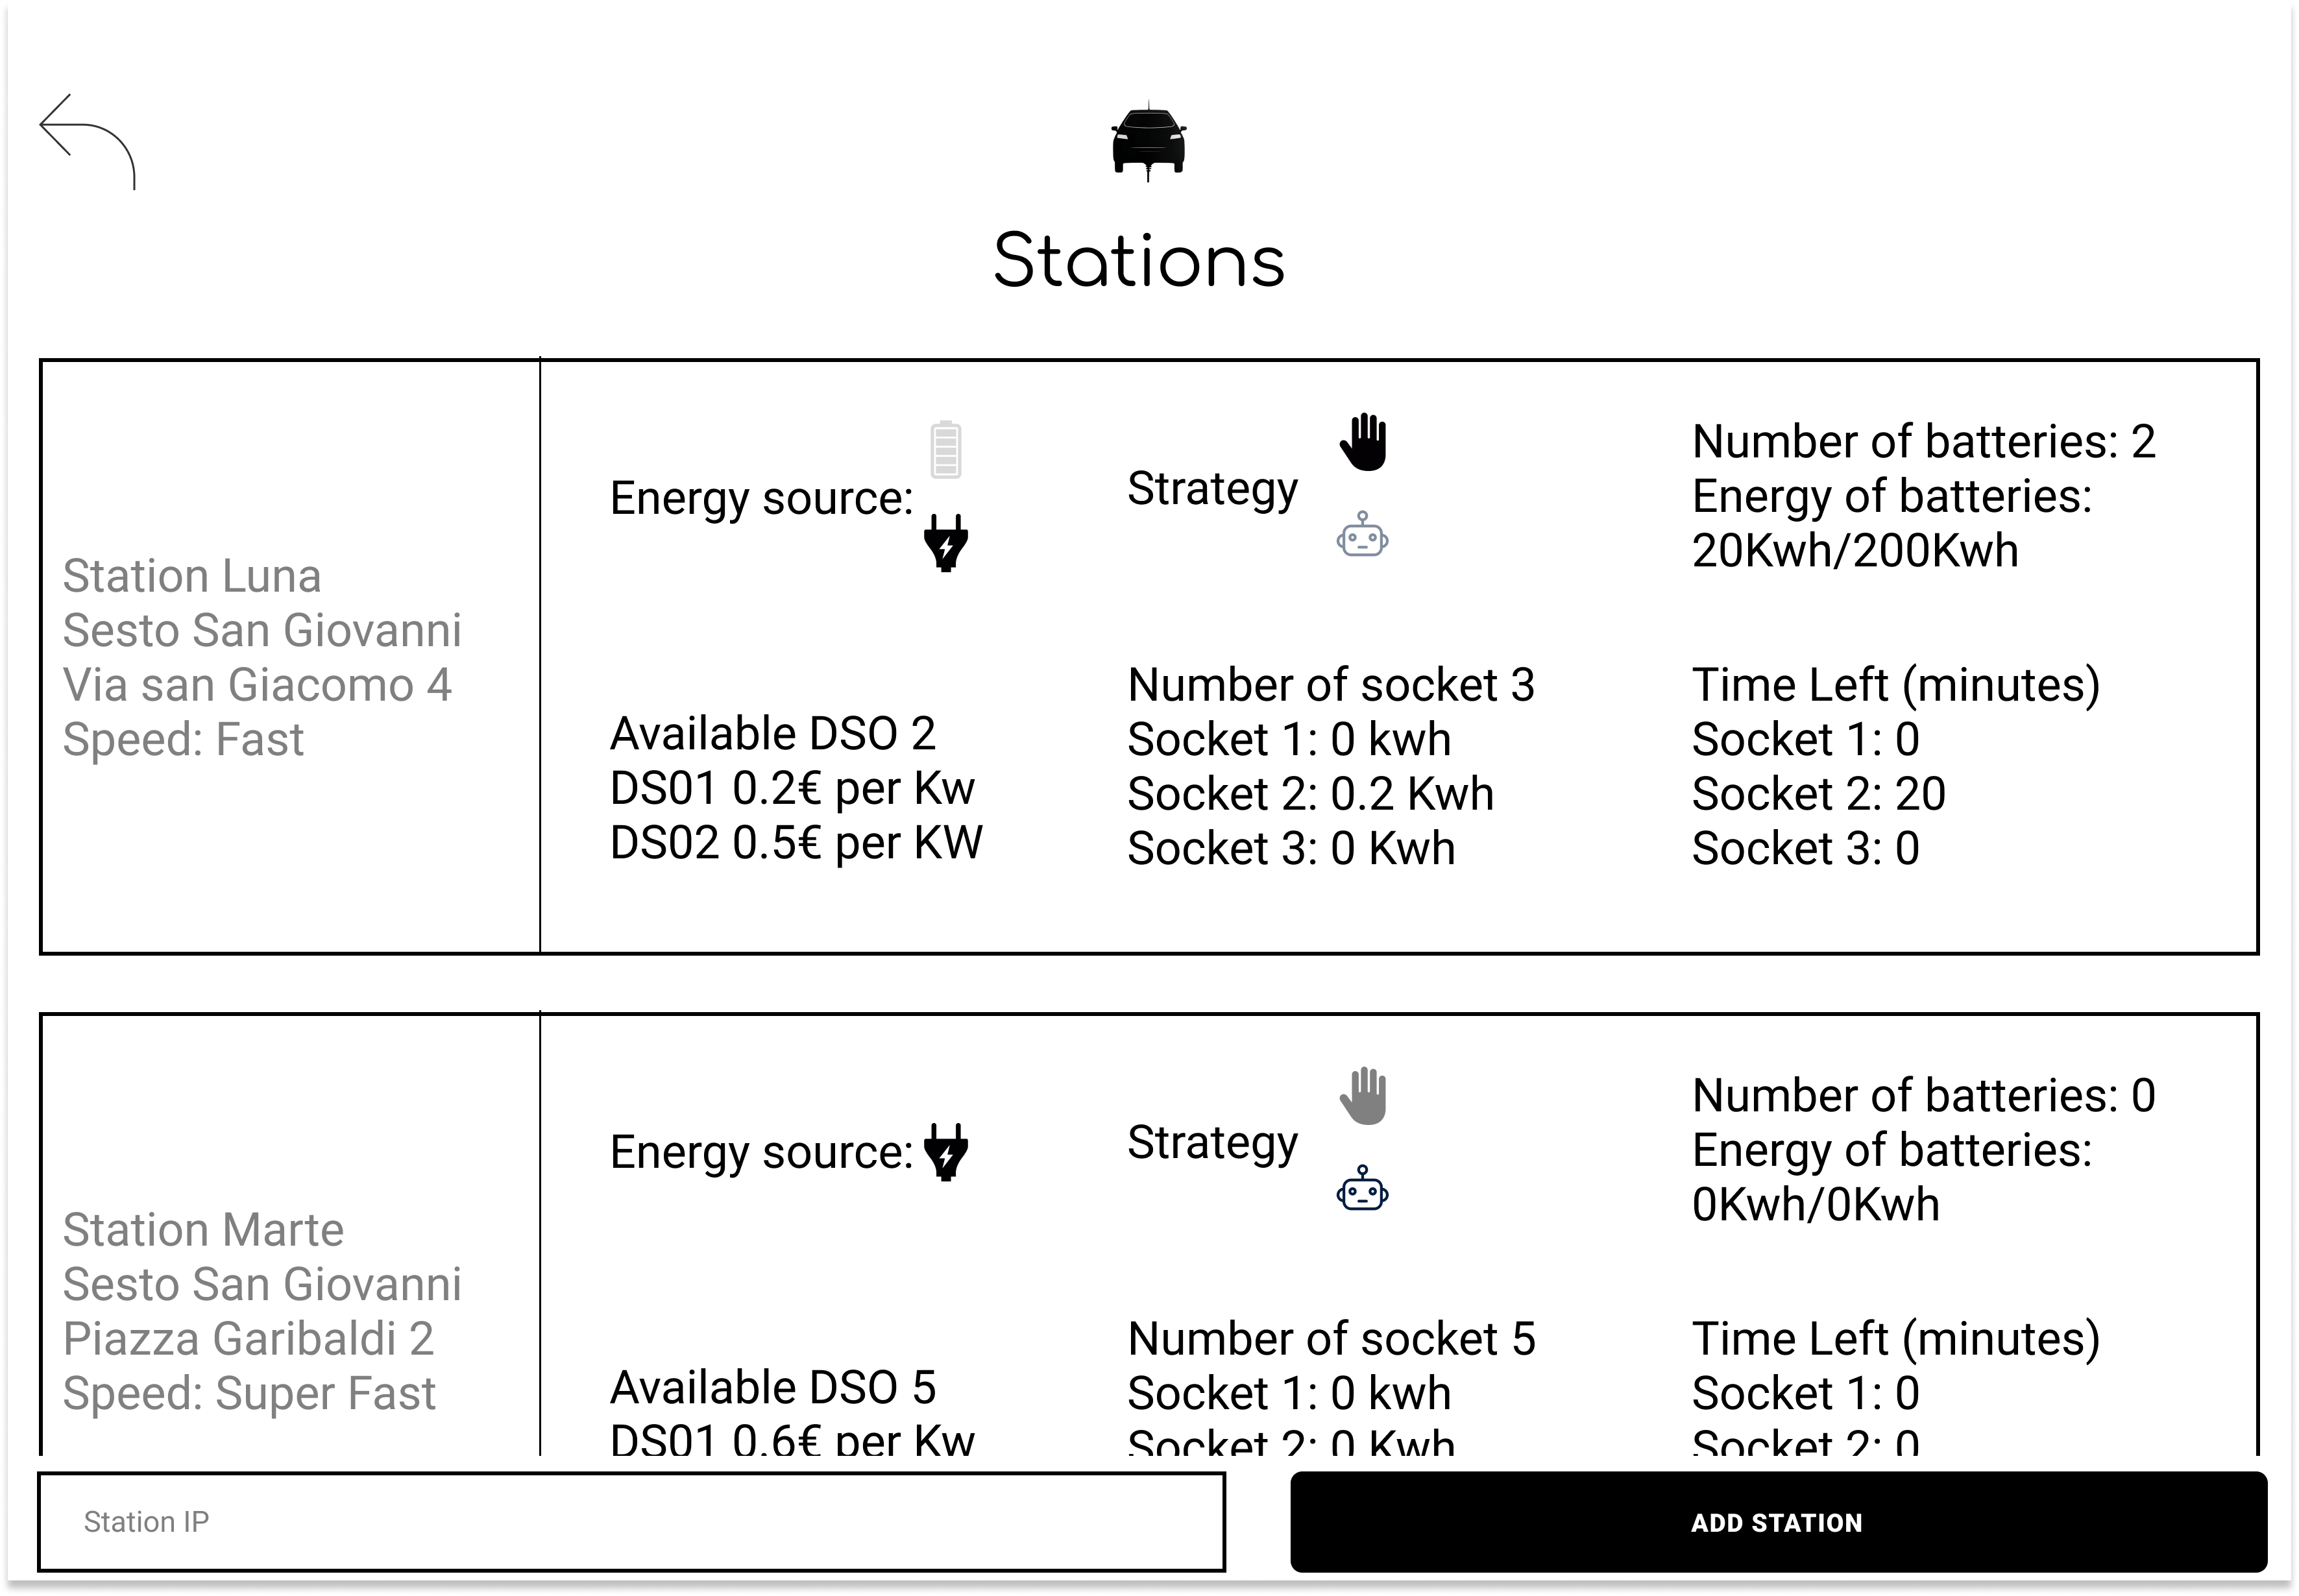
\includegraphics[keepaspectratio, width=15cm]{Mockup/CPMSSiteInterface/Add Station.png}
    \caption{\ac{CPO} manage stations}
    \label{cpo:Station}
\end{figure}
In this page all the information regarding the maintained stations are displayed. On the left the station location and name, on the right:
the number and capacity of battery, the available DSO and their prices, the number of socket, and for each active socket the current electricity usage and the time remaining for the charge.\\
The maintainer can change the energy source of the station by clicking the battery or plug icon (meaning battery or grid power is getting used). In the same fashion he/she can select the strategy by clicking either the hand or robot icon; the firs representing manual while the second automatic (opening the \hyperref[cpo:Station]{station page}).
The selected icon is bold while the other is greyed out. If no battery is available only the plug icon is displayed.\\
In this page it is also possible to add a new station to the system by adding its ip in the "station ip field" and pressing the add station button; the station will be added and the page refreshed displaying the new station and its data.\\
The user can return to the \hyperref[cpo:Homepage]{homepage} by pressing the backward arrow in the top left corner.

\subsubsection{Add Maintainer}
\begin{figure}[H]
    \centering
    \includegraphics[keepaspectratio, width=15cm]{Mockup/CPMSSiteInterface/Add Maintainer.png}
    \caption{\ac{CPO} add new \ac{CPO}Maintainers}
    \label{cpo:Maintainer}
\end{figure}
In this section the maintainer can add other maintainer to the station by simply creating the credentials(id and password) and pressing the add maintainer button, adding the new maintainer and loading the \hyperref[cpo:Homepage]{homepage}.\\
The user can return to the \hyperref[cpo:Homepage]{homepage} by pressing the backward arrow in the top left corner.
\subsection{Scenario UI}
The following table relate the different sequence diagrams with the corresponding user interfaces
\begin{table}[H]
    \begin{center}
        \begin{tabular}{|c||c|c|c|c|c|}
            \hline
            Sequence diagrams                                                                                   & Implemented by                                                         \\\hline
            \hyperref[fig:user-signs-up]{user-signs-up}                                                         & \ref{fig:Register}, \ref{fig:ConfirmReg}                               \\\hline
            \hyperref[fig:cpo-signs-up]{cpo-signs-up}                                                           & \ref{site:Register}, \ref{site:ConfirmReg}                             \\\hline
            \hyperref[fig:cpo-adds-cpms]{cpo-adds-cpms}                                                         & \ref{site:Homepage}                                                    \\\hline
            \hyperref[fig:cpo-removes-cpms]{cpo-removes-cpms}                                                   & \ref{site:Homepage}                                                    \\\hline
            \hyperref[fig:cpo-sets-revenue-percentage]{cpo-sets-revenue-percentage}                             & \ref{site:Homepage}                                                    \\\hline
            \hyperref[fig:cpo-sets-speciale-offer]{cpo-sets-speciale-offer}                                     & \ref{site:Homepage}                                                    \\\hline
            \hyperref[fig:user-executes-authorized-command]{user-executes-authorized-command}                   & \ref{fig:Login}, \ref{fig:FailedLogin}                                 \\\hline
            \hyperref[fig:user-searches-stations]{user-searches-stations}                                       & \ref{fig:Search}, \ref{fig:Results}.\ref{fig:Filters}                  \\\hline
            \hyperref[fig:user-books-charge]{user-books-charge}                                                 & \ref{fig:StationDetails}, \ref{pop:Booking},\ref{pop:BookingConfirmed} \\\hline
            \hyperref[fig:user-pays-charge]{user-pays-charge}                                                   & \ref{fig:myCharges}, \ref{pop:Pay}                                     \\\hline
            \hyperref[fig:user-cancels-charge]{user-cancels-charge}                                             & \ref{fig:myCharges}, \ref{pop:Delete}                                  \\\hline
            \hyperref[fig:cpomaintainer-executes-authorized-command]{cpomaintainer-executes-authorized-command} & \ref{cpo:Login}                                                        \\\hline
            \hyperref[fig:cpomaintainer-adds-cpomaintainer]{cpomaintainer-adds-cpomaintainer}                   & \ref{cpo:Homepage}, \ref{cpo:Maintainer}                               \\\hline
            \hyperref[fig:cpomaintainer-adds-stations]{cpomaintainer-adds-stations}                             & \ref{cpo:Homepage}, \ref{cpo:Station}                                  \\\hline
            \hyperref[fig:cpomaintainer-sets-station-strategy]{cpomaintainer-sets-station-strategy}             & \ref{cpo:Homepage}, \ref{cpo:Station}                                  \\\hline
            \hyperref[fig:cpomaintainer-sets-station-source]{cpomaintainer-sets-station-source}                 & \ref{cpo:Homepage}, \ref{cpo:Station}                                  \\\hline
        \end{tabular}
    \end{center}
    \caption{Linking table among sequences and user interfaces}
\end{table}
\clearpage